\documentclass[DynamicalBook]{subfiles}
\begin{document}
%




\setcounter{chapter}{0}%Just finished 0.


%------------ Chapter ------------%
\chapter{Wiring together dynamical systems}\label{chapter.1}

%-------- Section --------%
\section{Introduction}\label{sec.chap1_intro}

Here's a basic fact of life: \emph{things change}. And how things change most
often depends on how they currently are. This is the fundamental idea underlying all the various notions of \emph{dynamical
  system} that we will see in this book.

\begin{informal}\label{inf.dynam_sys2}
  A \emph{dynamical system} consists of:
  \begin{itemize}
  \item a notion of how things can be, called the \emph{states}, and
  \item a notion of how things will change given how they are, called the \emph{dynamics}.
  \end{itemize}
  The dynamics of a system might also depend on some free \emph{parameters} or \emph{inputs} that are imported from the environment, and
  we will often be interested in some particular \emph{variables} of the
  state that are \emph{exposed} or \emph{output} to the environment.
\end{informal}

You and I are big, complicated dynamical systems. Our bodies and minds are in
some particular configuration, and over time this configuration changes. We can
sense things --- seeing, touching, tasting --- and what we sense affects how our
bodies and minds change. Seeing a scary snake can make me recoil and feel fear,
but seeing a cute snake plushie can make me go over and start to pet it.
Some parts of me are also put back into the environment, like the expression on
my face. But not all of me is exposed in that way --- some things just go on in
my head.

This is the basic model of a dynamical system we will be working with in this
book.\footnote{At least until \cref{chapter.6}, where we will encounter other \emph{doctrines} of dynamical systems.} But to make the above informal definition precise, we need to answer
a number of questions:
\begin{itemize}
  \item What should a state be, really? Do we just have an abstract set of
    states, or could there be a continuum of states? Maybe there are some other
    structures that states can enter into which have to be respected by the
    dynamics, but aren't determined by them? \jaz{With this last sentence, I'm
      thinking of ``states as polynomial comonad aka category''. Not sure how to
    phrase it right.}
  \item What does it mean to change? Do we want to know precisely which state
    will be next if we know how things are? Or, maybe we will only have a guess
    at which state will come next? Or, maybe we'll just say how a state is
    tending to change, but not where it will end up?
  \item Do we always take in the same sort of parameters, or does it depend on
    how our system is placed in its environment? Should the dynamics vary
    continuously (or linearly, or some other way) in the choice of parameters?
\end{itemize}

Different people have decided on different answers to these questions for
different purposes. Here are three of the most widespread differents ways to answer those
questions:
\begin{enumerate}
  \item We'll assume the states form a discrete set, and that if we know the
    current state and our parameters, we know exactly what the next state will
    be. Such a system generally called a \emph{Moore machine} or \emph{deterministic automaton}.
  \item We'll assume the states form a continuum, but that we only know how a
    state is tending to change, not what the ``next'' state will be. Such a
    system is generally called a \emph{system of
      differential equations} --- the differential equations tells us the
    derivatives of the state variables: the way they are tending.
  \item We'll assume the states form a discrete set, but that we only have a
    guess at which state will follow from the current state. Such a system is generally
    called a \emph{Markov process}, or a \emph{Markov decision process}.
\end{enumerate}

We will call a way of answering these questions the \emph{theory} of dynamical
systems we are working in.
\begin{informal}\label{informal.doctrine2}
  A \emph{theory} of dynamical systems --- or a \emph{systems theory} for short --- is a particular way to answer the following
  questions about what it means to be a dynamical system:
  \begin{itemize}
  \item What does it mean to be a state?
  \item How should the output vary with the state --- discretely,
    continuously, linearly?
  \item Can the kinds of input a
    system takes in depend on what it's putting out, and how do they depend on it?
  \item What sorts of changes are possible in a given state?
  \item What does it mean for states to change.
  \item How should the way the state changes vary with the input?
  \end{itemize}
\end{informal}

Moore machines, differential equations, and Markov decision processes are each
dynamical systems understood in a different theory.
\begin{enumerate}
  \item A Moore machine is a dynamical system in a \emph{discrete and
      deterministic} systems theory.
  \item A system of differential equations is a dynamical system in a
    \emph{differential} systems theory.
  \item A Markov decision process is a dynamical system in a \emph{stochastic} systems theory.
\end{enumerate}

In most cases, mathematicians have assumed that that the kinds of parameters our systems take in
never change --- that our system will always interface with
    its environment in the same way. However, this assumption is quite
    restrictive; after all, I change the way I interface with my environment all
    the time. Every time I turn and face a new direction, I open myself up to
    new inputs. There are variations on all of the above systems theories which allow for the
    kinds of input to depend on what the system is putting out, but for most of this book, we will work with systems theories that pick a fixed sort of input.



The dynamical systems we will see in this book are \emph{open} in the sense that
they take in inputs from their environment and expose outputs back to their
environment. Because of this, our systems can interact with eachother. One
system can take what the other system outputs as part of its input, and the
other can take what the first outputs as part of its input. For example, when we
have a conversation, I take what I hear from you and use it to change how I
feel, and from those feelings I generate some speech which I output to the
world. You then take what I've said and do the same thing.

\begin{center}
  \jaz{Some wiring diagram of a conversation}
\end{center}

We call this way of putting together dynamical systems to make more complex
systems \emph{composition}.
\begin{informal}
  \emph{Composition} is the process by which some things are brought together to
  form bigger things.
\end{informal}

Functions can be composed by plugging outputs into inputs, and dynamical systems
can be composed by plugging in the variables of the states of some into the
parameters of others.

This book is all about composing dynamical systems. Because of this, we will use
the abstract language of composition: \emph{category theory}.
\begin{informal}
\emph{Category theory} is the abstract study of composition.
\end{informal}




%---- Subsection ----%
\subsection{Category Theory}\label{sec:category.theory}

We'll be using the language of category theory quite freely in this book, and so
we'll expect you to know the basics. These are the notions in category theory that you should look up if they are unfamiliar to you:
\begin{itemize}
\item What a category is.
\item What an isomorphism is.
\item What a functor is.
\item What a natural transformation is.
\item What a terminal and an initial object are.
\item What a product and a coproduct are.
\item What a monad is, and it will help if you also know what a comonad is.
  \item What a monoidal category is.
\end{itemize}

Good introductions to category theory abound. One place to start is \emph{An
  invitation to applied category theory} \cite{fong2019seven}. Another is
\emph{Notes on category theory} \cite{perrone2021notes}. For more mathematically inclined readers, see \cite{Riehl:Cats.in.context}.

We will be using cartesian categories quite a bit in the first few chapters.
\begin{definition}\label{def.cartesian_category}
  A category $\cat{C}$ is \emph{cartesian} if every two objects $A$ and $B$ in
  $\cat{C}$ have a product $A \times B$, and $\cat{C}$ has a terminal object
  $\ord{1}$. Equivalently, $\cat{C}$ is cartesian if for any finite set $I$ and
  $I$-indexed family $A_{(-)} : I \to \cat{C}$ of objects, there is a product
  $\prod_{i \in I} A_i$ in $\cat{C}$.

  A functor $F : \cat{C} \to \cat{D}$ between cartesian categories is said to be
  \emph{cartesian} if it preserves products and terminal objects, i.e.\ the
  map $(F\pi_A,\, F\pi_B) : F(A \times B) \to FA \times FB$ is an isomorphism
  for all $A$ and $B$, and the terminal morphism $F\ord{1} \to \ord{1}$ is an
  isomorphism.
\end{definition}

We will also use some more advanced category theory, like indexed
categories and double categories. However, you don't need to know them up front; we will introduce these concepts
as we use them.

While we're at it, here's some notation we'll use repeatedly throughout the book. The $n$th ordinal is denoted $\ord{n}$. It is defined to be the set
\[
\ord{n}\coloneqq\{1,2,\ldots,n\}.
\]
So $\ord{0}$ is the empty set, $\ord{1}$ is a one-element set, etc. We will also use
$$A + B$$
to mean the disjoint union (or coproduct) of sets.

%-------- Section --------%
\section{Deterministic and differential systems theories}

In this chapter, we will see how to wire together dynamical systems of all
different sorts. First, however, we start with two exemplary systems theories:

\begin{enumerate}
\item First, systems which we will call \emph{(discrete-time) deterministic
    systems}, which specify exactly which state the system will transition into
  given its current state and input parameters.
\item Second, systems which we will call \emph{differential systems}, which do
  not specify a ``next state'' but rather specify exactly how the state is
  tending to change in the moment, given the current state and input parameters.
\end{enumerate}


\subsection{Deterministic systems}\label{sec.deterministic_system}



A paradigmatic example of this sort of dynamical system is a clock.
\[
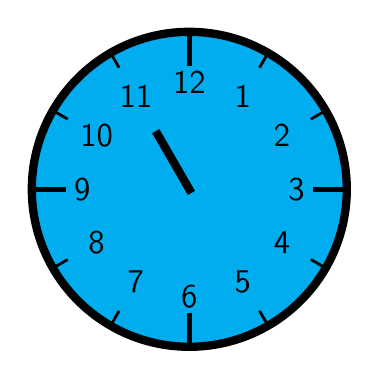
\begin{tikzpicture}[line cap=rect,line width=3pt]
\filldraw [fill=cyan] (0,0) circle [radius=2cm];
\foreach \angle [count=\xi] in {60,30,...,-270}
{
  \draw[line width=1pt] (\angle:1.8cm) -- (\angle:2cm);
  \node[font=\large] at (\angle:1.36cm) {\textsf{\xi}};
}
\foreach \angle in {0,90,180,270}
  \draw[line width=2pt] (\angle:1.6cm) -- (\angle:2cm);
\draw (0,0) -- (120:0.8cm);
\end{tikzpicture}
\]

Suppose that our clock has just an hour hand for now. Then we may collect all
the way things can be for the clock into a set of hours:
$$\Set{Hour} := \{1, 2, 3, 4, 5, 6, 7, 8, 9, 10, 11, 12\}.$$
This set $\Set{Hour}$ is the set of \emph{states} of our clock system.

If we know what hour it is, we also know what hour is coming next. So, this system has the following dynamics:
%
% :CUSTOM-ID: problem-with-drawing-mapsto-nicely
%
\begin{align}\label{eqn.tick}
  \fun{tick} : \Set{Hour} &\to \Set{Hour} \\\nonumber
                t &\mapsto \begin{cases} t + 1 &\mbox{if $t < 12$}\\ 1 &\mbox{if $t = 12$}  \end{cases}
\end{align}

By saying that the function $\fun{tick}$ is the dynamics for this system, what we mean is that this function sends the current state of the system to the next state it will have. Here's a sample of the dynamics of the clock. Say we started at the 10 o'clock state:
$$10 \xmapsto{\fun{tick}} 11 \xmapsto{\fun{tick}} 12 \xmapsto{\fun{tick}} 1 \To{\fun{tick}} 2
\xmapsto{\fun{tick}} \cdots$$

Ok, it's not the most dynamic of systems, but we have to start somewhere. If we want to
refer to the whole system at once, we can box it up and draw it like this:

\begin{equation}\label{eqn.clock_system_box}
\begin{tikzpicture}[oriented WD, every fit/.style={inner xsep=\bbx, inner ysep=\bby}, bbx = 1cm, bby =.5cm, bb min width=1cm, bb port length=4pt, bb port sep=1, baseline=(X.center)]
	\node[bb={0}{1}, fill=blue!10] (X) {$\Sys{Clock}$};
	\draw[label]
		node [right=2pt of X_out1] {$\Set{Hour}$}
		;
\end{tikzpicture}
\end{equation}
We imagine that the clock is going about its business inside the box, and
that is shows the hour it is currently displaying on the outgoing wire. This outgoing wire constitutes the clock's exposed variable, but we'll explain that more later.

One issue with our clock is that it doesn't tell us whether it is morning or
evening. Being morning or evening and going back and forth between them is another way that things might be and change, and hence we
can see it as its own two-state dynamical system with states
$$\Set{a.m./p.m.} = \{\const{a.m.}, \const{p.m.}\}.$$

However, rather than have this be an independent system, we want to consider it as a little addition to
our clock system, one that reads $\const{a.m.}$ or $\const{p.m.}$:
\begin{equation}\label{eqn.whole_clock}
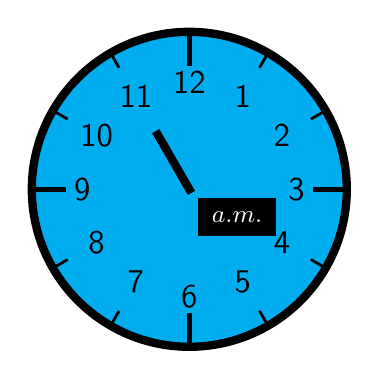
\begin{tikzpicture}[line cap=rect,line width=3pt, baseline=(bl)]
\coordinate (bl) at (0,0);
\filldraw [fill=cyan] (0,0) circle [radius=2cm];
\foreach \angle [count=\xi] in {60,30,...,-270}
{
  \draw[line width=1pt] (\angle:1.8cm) -- (\angle:2cm);
  \node[font=\large] at (\angle:1.36cm) {\textsf{\xi}};
}
\foreach \angle in {0,90,180,270}
  \draw[line width=2pt] (\angle:1.6cm) -- (\angle:2cm);
\draw (0,0) -- (120:0.8cm);
\node[draw, fill] at (330:.7cm) {\small${ \color{white}\const{a.m.} }$};
\end{tikzpicture}
\end{equation}
To connect the meridian to the clock means that the way the meridian changes should be based on the hour:
\begin{align}\label{eqn.next}
  \fun{next} : \Set{a.m./p.m.} \times \Set{Hour} &\to \Set{a.m./p.m.} \\\nonumber
               (\const{a.m.}, t) &\mapsto \begin{cases} \const{p.m.} &\mbox{if $t = 11$}\\ \const{a.m.} &\mbox{otherwise}  \end{cases} \\\nonumber
               (\const{p.m.}, t) &\mapsto \begin{cases} \const{a.m.} &\mbox{if $t = 11$}\\ \const{p.m.} &\mbox{otherwise}  \end{cases}
\end{align}
If it is $\const{a.m.}$ and the clock reads 8, then it will still be
$\const{a.m.}$ at the next tick; but if it is $\const{a.m.}$ and the clock reads 11, then the next tick will switch the meridian to $\const{p.m.}$.

Again, the thing to note about the dynamics of the $\const{a.m.}/\const{p.m.}$ system
is that they depend on what hour it is. The hour is imported as a \emph{parameter} for the
dynamics of the meridian system. We can draw the meridian system as a box like this:
\begin{equation}\label{eqn.am_pm_system_box}
\begin{tikzpicture}[oriented WD, every fit/.style={inner xsep=\bbx, inner ysep=\bby}, bbx = 1cm, bby =.5cm, bb min width=1cm, bb port length=4pt, bb port sep=1, baseline=(X.center)]
	\node[bb={1}{1}, fill=blue!10] (X) {$\Sys{Meridian}$};
	\draw[label]
		node [left=2pt of X_in1] {$\Set{Hour}$}
		node [right=2pt of X_out1] {$\Set{a.m./p.m.}$}
		;
\end{tikzpicture}
\end{equation}
We have the $\Set{a.m./p.m.}$ wire coming out, which carries the information of
whether it is $\const{a.m.}$ or $\const{p.m.}$, just like the clock. But we also
have a wire coming in, which carries the hour that we need as a parameter for
our dynamics.


We can now express our whole clock \eqref{eqn.whole_clock} by wiring together
our bare clock \eqref{eqn.clock_system_box} and the $\const{a.m.}/\const{p.m.}$ system:

\begin{equation}\label{eqn.whole_clock_system_box}
\begin{tikzpicture}[oriented WD, every fit/.style={inner xsep=\bbx, inner ysep=\bby}, bbx = .3cm, bby =.3cm, bb min width=.5cm, bb port length=2pt, bb port sep=1, baseline=(Y.center)]
	\node[bb={1}{1}, fill=blue!10] (X1) {$\Sys{Meridian}$};
  	\node[bb={0}{1}, fill=blue!10, below=2 of X1] (X2) {$\Sys{Clock}$};
	\node[bb={0}{2}, fit={($(X1.north west)+(-2,1)$) ($(X1.north east)+(2,1)$) ($(X2.south)+(0,-3)$)}] (Y) {};
  \node[above=0pt of Y.south] (Label) {$\Sys{ClockWithDisplay}$};
	\draw (X1_out1) to (Y_out1);
  \draw let \p1=(X1.south west), \p2=(X2.north east), \n1=\bbportlen, \n2=\bby in
    (X2_out1) to[in=0] (\x2 + \n1, \y2 + \n2) -- (\x1 - \n1, \y2 + \n2) to[out=180] (X1_in1);
  \draw (X2_out1) to (Y_out2);
	\draw[label]
		node [right=2pt of Y_out1] {$\Set{a.m./p.m.}$}
		node [right=2pt of Y_out2] {$\Set{Hour}$}
		;
\end{tikzpicture}
\end{equation}

We've put both our systems $\Sys{Meridian}$ and $\Sys{Clock}$ into this bigger box with two outgoing wires. We didn't just dump these systems in the bigger box; we connected them up to each other and the outgoing wires. The resulting system has states
$$\Set{HoursWithDisplay} := \Set{Hour} \times \Set{a.m./p.m.}$$
each of which is a pair, e.g.\ $(11, \const{a.m.})$, consisting of an hour and a meridian reading.
They update in a combined way, by using the hour shown on the clock face as the
parameter we need for the $\Sys{Meridian}$ system; this is expressed by having a wire from the output of $\Sys{Clock}$ to the input of $\Sys{Meridian}$. In full, the
dynamics looks like this:
\begin{align*}
  \fun{tick'} :\Set{HoursWithDisplay} &\to \Set{HoursWithDisplay} \\
  (t, m) &\mapsto (\fun{tick}(t), \fun{next}(t, m))
\end{align*}
where $\fun{tick}$ and $\fun{next}$ are as in \eqref{eqn.tick} and \eqref{eqn.next}.

\begin{exercise}
  Convince yourself that the combined system really does behave like the clock with $\const{a.m.}/\const{p.m.}$ display should.
\end{exercise}

Now that we have a working clock, we can use it for systems that need to know
the time. For example, consider a diner that opens at $7 \const{a.m.}$ and
closes at $10 \const{p.m.}$. The states of this diner are
$$\Set{DinerState} = \{\const{open}, \const{closed}\}.$$
The diner's dynamics are then
\begin{align*}
  \fun{dinerDynamics} : \Set{DinerState} \times \Set{HoursWithDisplay} &\to \Set{DinerState} \\
  (\const{open}, (10, \const{p.m.})) &\mapsto \const{closed} \\
  (\const{closed}, (7, \const{a.m.})) &\mapsto \const{open} \\
  (s, (t, m)) &\mapsto s \quad\mbox{otherwise.}
\end{align*}

Again, we can represent the diner by this box:
\begin{equation}\label{eqn.diner_system_box}
\begin{tikzpicture}[oriented WD, every fit/.style={inner xsep=\bbx, inner ysep=\bby}, bbx = 1cm, bby =.5cm, bb min width=1cm, bb port length=4pt, bb port sep=1, baseline=(X.center)]
	\node[bb={2}{1}, fill=blue!10] (X) {$\Sys{Diner}$};
	\draw[label]
		node [left=2pt of X_in1] {$\Set{a.m./p.m.}$}
		node [left=2pt of X_in2] {$\Set{Hour}$}
		node [right=2pt of X_out1] {$\Set{DinerState}$}
		;
\end{tikzpicture}
\end{equation}
This time, we have two wires coming in, corresponding to the two parameters we
need for the diner system: the hour and the
meridian.

Assuming that the diner has a clock on its wall which it uses to decide whether
to open or close, the full diner system would be given by wiring the clock with display into
those input wires:
\begin{equation}\label{eqn.diner_system_box}
\begin{tikzpicture}[oriented WD, every fit/.style={inner xsep=\bbx, inner ysep=\bby}, bbx = 1cm, bby =.5cm, bb min width=1cm, bb port length=4pt, bb port sep=1, baseline=(Outer.center)]
  \node[bb={0}{2}, fill=blue!10](Clock) {$\Sys{ClockWithDisplay}$};
  \node[bb={2}{1}, fill=blue!10, right=of Clock] (Diner) {$\Sys{Diner}$};

  \node[bb={0}{1}, fit={(Clock) (Diner)}] (Outer) {};

  \draw (Clock_out1) to (Diner_in1);
  \draw (Clock_out2) to (Diner_in2);
  \draw (Diner_out1) to (Outer_out1);

  \draw[label] node [right=2pt of Outer_out1] {$\Set{DinerState}$};
\end{tikzpicture}
\end{equation}
If we want to, we can peak into the clock with display and see that it is itself
made out of a clock wired to a display:
\begin{equation}\label{eqn.diner_system_box}
\begin{tikzpicture}[oriented WD, every fit/.style={inner xsep=\bbx, inner ysep=\bby}, bbx = 1cm, bby =.3cm, bb min width=1cm, bb port length=4pt, bb port sep=1, baseline=(Outer.center)]
	\node[bb={1}{1}, fill=blue!10] (X1) {$\Sys{Meridian}$};
  	\node[bb={0}{1}, fill=blue!10, below=2 of X1] (X2) {$\Sys{Clock}$};
	\node[dashed, bb={0}{2}, fit={($(X1.north west)+(0,1)$) ($(X1.north east)+(0,1)$) ($(X2.south)+(0,-3)$)}] (Clock) {};
  \node[above=0pt of Clock.south] (Label) {$\Sys{ClockWithDisplay}$};
	\draw (X1_out1) to (Clock_out1);
  \draw let \p1=(X1.south west), \p2=(X2.north east), \n1=\bbportlen, \n2=\bby in
    (X2_out1) to[in=0] (\x2 + \n1, \y2 + \n2) -- (\x1 - \n1, \y2 + \n2) to[out=180] (X1_in1);
  \draw (X2_out1) to (Clock_out2);
  \node[bb={2}{1}, fill=blue!10, right=of Clock] (Diner) {$\Sys{Diner}$};

  \node[bb={0}{1}, fit={(Clock) (Diner)}] (Outer) {};

  \draw (Clock_out1) to (Diner_in1);
  \draw (Clock_out2) to (Diner_in2);
  \draw (Diner_out1) to (Outer_out1);

  \draw[label] node [right=2pt of Outer_out1] {$\Set{DinerState}$};
\end{tikzpicture}
\end{equation}

These examples are simple, but it doesn't take much more to get to some truly
amazing phenomena. Consider this system: we have an infinite tape with a
read-head at some integer position. On this infinite tape, we will write the symbols
$a$, $b$, $c$, or $d$, or we will leave it blank: $\_$. Together, the state
of the tape and the position of the read-head have states pairs $(\fun{T}, n)$ consisting of a
function $\fun{T} : \zz \to \{a, b,c,d,\_\}$, telling us what symbol $\fun{T}(i)$ is found at
position $i$ of the tape, and a position $n$ of the read-head:
\begin{align*}
  \Set{Symbol} &= \{a, b,c,d,\_\}\\
  \Set{Tape} &= \Set{Symbol}^{\zz}\\
  \Set{Head} &= \zz
\end{align*}
The parameters that this system needs in order to change are a move-command and a
write-command. The move-command will be either move left or move right, encoded as $-1$ or $1$ respectively, and the write command will be one of the
symbols that can be written on the tape:
\[
  \Set{Move}=\{-1,1\}\qqand
  \Set{Write} = \{a,b,c,d,\_\}.
\]

The way this system changes is by writing the write command to the tape at the current
position, and then moving according to the move command. As a function, this is:
\begin{align*}
  \fun{execute} : \Set{Head} \times \Set{Tape} \times \Set{Move} \times \Set{Write} &\to \Set{Head} \times \Set{Tape}\\
  (n, i\mapsto \fun{T}(i), d, s) &\mapsto \left( n + d, i \mapsto \begin{cases} \fun{T}(i) &\mbox{if $i \neq n$} \\ s &\mbox{if $i = n$} \end{cases} \right).
\end{align*}

We can imagine that the system exposes the tape and the symbol under its read head. We can box this system up and draw it like so:
\begin{equation}\label{eqn.turing_box}
\begin{tikzpicture}[oriented WD, every fit/.style={inner xsep=\bbx, inner ysep=\bby}, bbx = 1cm, bby =.5cm, bb min width=1cm, bb port length=4pt, bb port sep=1, baseline=(Tape.center)]
\node[bb={2}{2}, fill=blue!10] (Tape) {$\Sys{Tape Machine}$};
\draw[label]
  node[left=2pt of Tape_in1] {$\Set{Move}$}
  node[left=2pt of Tape_in2] {$\Set{Write}$}
  node[right=2pt of Tape_out1] {$\Set{Tape}$}
  node[right=2pt of Tape_out2] {$\Set{Symbol}$}
;
\end{tikzpicture}
\end{equation}

Now, we need one more simple ingredient to get our system going; a mysterious system of the
form:
\begin{equation}\label{eqn.turing_box2}
\begin{tikzpicture}[oriented WD, every fit/.style={inner xsep=\bbx, inner ysep=\bby}, bbx = 1cm, bby =.5cm, bb min width=1cm, bb port length=4pt, bb port sep=1, baseline=(Box.center)]
\node[bb={1}{2}, fill=blue!10] (Box) {$\Sys{Mystery Box}$};
\draw[label]
  node[right=2pt of Box_out1] {$\Set{Move}$}
  node[right=2pt of Box_out2] {$\Set{Write}$}
  node[left=2pt of Box_in1] {$\Set{Symbol}$}
;
\end{tikzpicture}
\end{equation}

We can see that our mystery box will take in a symbol and put out a move command
and a write command. The way our mystery box behaves is rather mysterious. It has seven states $S = \{1, 2, 3, 4, 5, 6, \text{end}\}$, and its update rule is given by the following table,
where the entry in the row $i$ and the column $s$ is written $(m,w):s'$ to express the
move command $m$, the write command $w$, and the next state $s'$ that our
mysterious system transitions to when input the symbol $i$ in state $s$:
\begin{equation}\label{eqn.turing_machine}
  \begin{tabular}{|c|c|c|c|c|c|c|}
    \hline
     & 1 & 2 & 3 & 4 & 5 & 6 \\\hline
    a & (-1, b):1 & (1, a):1 & (-1, b):3  & (1, b):2 & (-1, b):6 & (-1, b):4 \\\hline
   b & (-1, a):1 & (1, a):2 & (-1, b):5  & (1, a):4 & (1, a):6 & (1, a):5 \\\hline
   c & (1, d):2 & (1, d):2 & (-1, c):5 & (1,d):4 & (1, c):5 & (1, a):1 \\\hline
   d & (-1, c):1 & (1, a):5 & (-1, c):3 & (1,d):5 & (-1, b):3 & end \\\hline
  \end{tabular}
\end{equation}
The $\text{end}$ state always transitions to itself. Mysterious indeed. But when we wire the two together, magic happens!

\begin{equation}\label{eqn.full_turing_machine}
\begin{tikzpicture}[oriented WD, every fit/.style={inner xsep=\bbx, inner ysep=\bby}, bbx = 1cm, bby =.5cm, bb min width=1cm, bb port length=2pt, bb port sep=1, baseline=(Outer.center)]
  \node[bb={1}{2}, fill=blue!10](Box) {$\Sys{Mystery Box}$};
  \node[bb={2}{2}, fill=blue!10, right=of Box] (Tape) {$\Sys{Tape Machine}$};

  \node[bb={0}{0}, fit={($(Tape.south east) + (0, -2)$) ($(Box.north west) + (0, 1)$)}] (Outer) {};
  \node[above=0pt of Outer.south] (Label) {$\Sys{Universal Turing Machine}$};

  \draw (Box_out1) to (Tape_in1);
  \draw (Box_out2) to (Tape_in2);

  \draw (Tape_out1) to (Outer.east|-Tape_out1);
  \draw (Tape_out2) to (Outer.east|-Tape_out2);

  \draw let \p1=(Tape.south east), \p2=(Box.south west), \n1=\bbportlen, \n2=\bby in
    (Tape_out2) to[in=0] (\x1 + \n1, \y1 - \n2 - 1) -- (\x2 - \n1, \y2 - \n2 - 1) to[out=180] (Box_in1);
\end{tikzpicture}
\end{equation}
This is a universal Turing machine, i.e.\ when we encode everything into this strange alphabet, it is capable of arbitrarily complex calculation!
\slogan{Even simple systems can
have very interesting behavior\\ when plugged in to the right environment.}

%%
%% :CUSTOM_ID:cite-this.turing_machine
%%
That's a lot of informal definitions, we are ready for something precise:
\begin{definition}\label{def.deterministic_system}
  A \emph{deterministic system} $\Sys{S}$, also written as
  $$\lens{\update{S}}{\expose{S}} : \lens{\State{S}}{\State{S}} \leftrightarrows \lens{\In{S}}{\Out{S}},$$
  consists of:
  \begin{itemize}
    \item a set $\State{S}$ of \emph{states};
    \item a set $\Out{S}$ of \emph{values for exposed variables}, or \emph{outputs}
      for short;
    \item a set $\In{S}$ of \emph{parameter values}, or \emph{inputs} for short;
    \item a function $\expose{S} : \State{S} \to \Out{S}$, the \emph{exposed variable of state} or
      \emph{expose} function, which takes a state to the output it yields; and
    \item a function $\update{S} : \State{S} \times \In{S} \to \State{S}$, the \emph{dynamics} or
      \emph{update} function which takes a state and a parameter and gives the
      next state.
  \end{itemize}
  We refer to the pair $\lens{\In{S}}{\Out{S}}$ of exposed variable and parameter values as
  the \emph{interface} of the system.

We can interpret this definition in any cartesian category $\cat{C}$ by taking $\State{S}$, $\Out{S}$ and $\In{S}$ to be objects of $\cat{C}$ and $\update{S}$ and $\expose{S}$ to be maps in $\cat{C}$; here, we
have have used the cartesian category $\Cat{Set}$ of sets.
\end{definition}

\begin{remark}
  Deterministic systems are also known as \emph{Moore machines} in the
  literature. If the output set is taken to be $\{\const{true},
  \const{false}\}$, then they are known as \emph{deterministic automata}.

  Often, these definitions also include a \emph{start state} $s_0 \in \State{S}$
  as part of the data. We don't do this.
\end{remark}

\begin{example}\label{ex.clock_system}
  The $\Sys{Clock}$ system can be seen as a deterministic system with:
  $$\lens{\fun{tick}}{\id} : \lens{\Set{Hour}}{\Set{Hour}} \fromto \lens{\{\ast\}}{\Set{Hour}}.$$
  In other words, it consists of
  \begin{itemize}
  \item State set $\State{Clock} = \Set{Hour} =\{1,2,\ldots,12\}$.
  \item Output set $\Out{Clock} = \Set{Hour}$.
  \item Input set $\In{Clock} = \{\ast\}$, a one element set.
  \item Readout function $\expose{Clock} = \id_{\Set{Hour}}$.
  \item update function $\update{Clock} : \Set{Hour} \times \{\ast\} \to \Set{Hour}$
    defined by $\update{Clock}(t, \ast) = \fun{tick}(t)$.
  \end{itemize}
\end{example}

\begin{example}\label{ex.moore_machine}
  Not only is the term \emph{Moore machine} is used for the mathematical notion of
  deterministic system we've just presented, but it is also used for actual,
  real-life circuits which are designed on that principle.

  For example, suppose that a wire carries the signals $\Set{Wire} =
  \{\const{high}, \const{low}\}$. We can see a deterministic system $\Sys{M}$
  with input $\In{M} = \Set{Wire}^n$ and $\Out{M} = \Set{Wire}^k$ as a circuit
  with $n$ incoming wires and $k$ outgoing wires.\footnote{Of course, the notion
  of ``incoming'' and ``outgoing'' wires are ways we think about the circuit in
  design terms. Circuits aren't actually directed in this way. We'll think about
undirected notions of system in \cref{chapter.2}.} The state then describes the
state of all the internal wires (and capacitors, etc.) in the circuit. We would wire up these systems by literally wiring them together.

\jaz{I would like to add an example of an implementation of a Moore machine into
  a circuit.}
%%
%%  :CUSTOM-ID:moore-machine-example
%%
\end{example}

Note that when we say that a system doesn't have any parameters, as in \cref{ex.clock_system}, we don't take the
parameter set to be empty but instead take it to have a single dummy value $\{*\}$, the one-element ``hum of existence''. In other words, having ``no parameters'' really means that the parameters are unchanging, or that there is no way to change the value of the parameters.

Also, we are just exposing the whole state with the system in \cref{ex.clock_system}. There is nothing preventing our systems
from exposing their whole state (which means $\State{S} = \Out{S}$ and $\expose{S} = \id$), but often some aspects of the state are private, i.e.\ not exposed for use by other systems.

\begin{exercise}\label{exc.clock_meridian_diner}
  Write out the clock and meridian systems from \eqref{eqn.tick} and \eqref{eqn.next} in terms of
  \cref{def.deterministic_system}. Really, this amounts to noticing which sets
  are the sets of states, which are the sets of inputs, and what (implicitly)
  are the sets of outputs.
\end{exercise}

\begin{example}[SIR model]\label{ex.SIR_model_discrete}
  The set of states for a deterministic system doesn't need to be finite. The $\Sys{SIR}$ model
  is an epimediological model used to study how a disease spreads through a
  population. ``SIR'' stands for ``susceptible'', ``infected'', and, rather
  ominously, ``removed''. This model is usually presented as a system of
  differential equations --- what we will call a differential system --- and we will see it in that form in \cref{ex.SIR_model_diff}.
  But we can see a discrete approximation to this continuous model as a
  deterministic system.

  A state of the $\Sys{SIR}$ model is a choice of how many people are susceptible, how
  many are infected, and how many are removed. That is,
  $$\State{SIR} = \left\{\begin{bmatrix} s \\ i \\ r \end{bmatrix}\; \middle|\; s,\, i,\, r\in \rr\right\} \cong \rr^3.$$
  is a 3-place vector of real numbers. We will again expose the whole state, so
  $\Out{SIR} = \State{SIR}$ and $\expose{SIR} = \id$.

  The idea behind the $\Sys{SIR}$ model is that if a susceptible person comes in
  contact with an infected person, then they have a chance of becoming infected
  too. And, eventually, infected persons will be removed from the model, either
  by recovering (a gentler way to read the ``R'') or by dying. So we need two
  parameters: the rate $a$ of infection and the rate $b$ of removal:
  $$\In{SIR} = \left\{\begin{bmatrix} a \\ b \end{bmatrix}\, \middle|\, a,\, b \in \rr\right\} = \rr^2.$$

  Now, we can show how a population will develop according to this model by
  defining the update function:
  \begin{align}\label{eqn.SIR_model_discrete}
    \update{SIR} : \State{SIR} \times \In{SIR} &\to \State{SIR}\\
    \left( \begin{bmatrix} s\\ i\\ r\\ \end{bmatrix},\, \begin{bmatrix}a \\ b \end{bmatrix} \right) &\mapsto \begin{bmatrix}s - a s i \\ i + a s i - b  i \\ r + b i \end{bmatrix}
  \end{align}

\end{example}

\begin{example}\label{ex.transition_diagram_discrete}
  If a deterministic system has a small finite set of states, then we can draw it
entirely as a \emph{transition diagram}:

\[
\begin{tikzpicture}
	\node[draw] {
  \begin{tikzcd}[column sep=small]
  	\LMOO{1}{a}\ar[rr, dgreen, thick, bend left]\ar[loop left, thick, orange]&&
  	\LMOO{2}{b}\ar[ll, thick, orange, bend left]\ar[dl, bend left, thick, dgreen]\\&
  	\LMOO{3}{b} \ar[ul, thick, orange, bend left] \ar[loop left, thick, dgreen]
  \end{tikzcd}
  };
\end{tikzpicture}
\]
Note that every node has an orange and a green arrow emanating from it, but that there are no rules on how many arrows point to it.

This diagram describes the following system $\Sys{S}$:
  $$\lens{\update{S}}{\expose{S}} : \lens{\{1, 2, 3\}}{\{1, 2, 3\}} \leftrightarrows \lens{\{{\color{dgreen} \const{green},\, {\color{orange} \const{orange}}}\}}{\{a, b\}}.$$
That is, we have
\begin{itemize}
\item $\State{S} = \{1, 2, 3\}$.
\item $\In{S} = \{{\color{dgreen} \const{green},\, {\color{orange} \const{orange}}}\}$,
\item $\Out{S} = \{a, b\}$,
\item \[\begin{aligned}
        \expose{S} : \State{S} &\to \Out{S} \\
        1 &\mapsto a \\
        2 &\mapsto b \\
        3 &\mapsto b \\~\\~\\~\\
      \end{aligned} \quad\quad\quad\quad
 \begin{aligned}
        \update{S} : \State{S} \times \In{S} &\to \State{S} \\
        (1, {\color{dgreen} \const{green}}) &\mapsto 2 \\
        (1, {\color{orange} \const{orange}}) &\mapsto 1 \\
        (2, {\color{dgreen} \const{green}}) &\mapsto 3 \\
        (2, {\color{orange} \const{orange}}) &\mapsto 1 \\
        (3, {\color{dgreen} \const{green}}) &\mapsto 3 \\
        (3, {\color{orange} \const{orange}}) &\mapsto 1
      \end{aligned}
      \]
\end{itemize}

To draw a transition diagram of a system $\Sys{S}$, we draw each state $s \in
\State{S}$ as a bubble filled with the label $\expose{S}(s)$, and for each
parameter $i \in \In{S}$ we draw an arrow from $s$ to $\update{S}(s, i)$ and label it by $i$. For a
diagram like this to be a transition diagram, every node must have exactly one edge
leaving it for each parameter.
\end{example}

\begin{exercise}
  Draw the $\Sys{Clock}$ system (\cref{ex.clock_system}) as a transition diagram.
\end{exercise}

\begin{example}[Deterministic Finite Automata]\label{ex.dfa}
  A \emph{deterministic finite automaton} (DFA) is a simple model of computation.
  Given our definition of deterministic system, DFAs are easy enough to define:
  they are just the deterministic systems with finitely many states whose output values are either
  $\const{accept}$ or $\const{reject}$.

  This means that the exposed variable of state $\expose{S} : \State{S} \to
  \{\const{accept},\, \const{reject}\}$ is a boolean valued function. We say a
  state $s$ is an \emph{accept state} if $\expose{S}(s) = \const{accept}$, and a
  \emph{reject state} if $\expose{S}(s) = \const{reject}$.

  The idea is that a DFA is a question answering machine. Given a starting state
  $s_0$ and a sequence of input values $i_1, \ldots, i_n$, we get a sequence of
  states by $s_{t+1}:= \update{S}(s_t, i_t)$. The answer to the question is
  ``yes'' if $s_n$ is an accept state, and ``no'' if $s_n$ is a reject state.
\end{example}

There is an important special case of deterministic systems which appear very
commonly in the literature: the \emph{closed} systems. These are the systems
which have no parameters, and which expose no variables. They are closed off
from their environment, and can't be wired into any other systems.

As mentioned after \cref{ex.clock_system}, when we say ``no'' in this way --- no parameters, no variables --- we should be
careful with what we mean exactly. We mean that there is no \emph{variation} in
the parameters or variables, that they are trivial. That is, we make the
following definition.
\begin{definition}
  We say that a deterministic system $\Sys{S}$ as ``no inputs'' if $\In{S}$ has a single element, and has ``no outputs'' if $\Out{S}$ has a single element. We say that $\Sys{S}$ is \emph{closed} if it has no inputs and no outputs: both $\In{S}$ and
  $\Out{S}$ have only one element
  \[\In{S}\cong\{*\}\cong\Out{S}.\]
\end{definition}

\begin{exercise}
Show that to give a closed system
\[\lens{\update{S}}{\expose{S}}\colon\lens{\State{S}}{\State{S}}\fromto\lens{\{*\}}{\{*\}},\]
one just needs to choose a set $\State{S}$ and an update function $\update{S} :  \State{S} \to \State{S}$.
\end{exercise}

Given that we are mostly interested in how systems wire together, it may seem
strange to draw attention to the closed systems that \emph{can't} be wired into
anything else. But we will often end up with a closed system as the result of
wiring together some systems.

For example, suppose we have an $\Sys{Agent}$ acting within a
$\Sys{Environment}$. The agent will take an action, and the evironment will
respond to that action. Depending on the action taken and response given, the
agent and the environment will update their states. We can model this by the
following wiring diagram:
\[
\begin{tikzpicture}[oriented WD, every fit/.style={inner xsep=\bbx, inner ysep=\bby}, bbx = 1cm, bby =.5cm, bb min width=1cm, bb port length=2pt, bb port sep=1, baseline=(Outer.center)]
  \node[bb={1}{1}, fill=blue!10](Box) {$\Sys{Agent}$};
  \node[bb={1}{1}, fill=blue!10, right=of Box] (Tape) {$\Sys{Environment}$};

  \node[bb={0}{0}, fit={($(Tape.south east) + (0, -2)$) ($(Box.north west) + (0, 1)$)}] (Outer) {};
  \node[above=0pt of Outer.south] (Label) {$\Sys{Closed\ Agent/Environment\ Model}$};

  \draw (Box_out1) to (Tape_in1);


  \draw let \p1=(Tape.south east), \p2=(Box.south west), \n1=\bbportlen, \n2=\bby in
    (Tape_out1) to[in=0] (\x1 + \n1, \y1 - \n2 - 1) -- (\x2 - \n1, \y2 - \n2 - 1) to[out=180] (Box_in1);
\end{tikzpicture}
\]

To model this as a closed system is to think --- or pretend --- that the our model
of the $\Sys{Agent}$ and the $\Sys{Environment}$ includes all possible external
parameters, that it is well isolated from its own environment.

\begin{exercise}
What would happen to a system $\Sys{S}$ if its set of parameters or output values were actually empty sets? Let's find out.
\begin{enumerate}
	\item Suppose $\In{S}=\varnothing$. Explain the content of a deterministic system \[\lens{\update{S}}{\expose{S}}\colon\lens{\State{S}}{\State{S}}\fromto\lens{\varnothing}{\{*\}}.\]
	\item Suppose $\Out{S}=\varnothing$. Explain the content of a deterministic system \[\lens{\update{S}}{\expose{S}}\colon\lens{\State{S}}{\State{S}}\fromto\lens{\{*\}}{\varnothing}.
	\qedhere
\]
\end{enumerate}
\end{exercise}



\subsection{Differential systems}\label{sec.differential_system}

\begin{quote}
  \emph{La nature ne fait jamais des sauts} - Liebniz
\end{quote}

A quirk of modeling dynamical systems as determinstic systems is that
determinstic systems lurch from one state to the next. In life, there are no
next moments. Time, at least at human scales and to a first approximation, flows
continuously.

Instead of modelling the ``next'' state a system will be in, we can model
\emph{how the system is tending to change}, in the moment. In order to do this,
we need to make concession in the way we model the states of our system: we must
assume they form a continuum themselves.

For example, suppose we are studying a population of $\Sys{Rabbits}$. We can
measure the rate at which rabbits are born, and the rate they die. Then the
population changes according to these rates. We can express this dependency of
the change in population on certain rates with a differential equation:
\[
\frac{dr}{dt} = \const{b}_{\Sys{Rabbits}} \cdot r - \const{d}_{\Sys{Rabbits}}
\cdot r
\]
where $r \in \rr$ is the population of rabbits (considered as a real number for
convenience), and the rates $\const{b}_{\Sys{Rabbits}}$ and
$\const{d}_{\Sys{Rabbits}}$. The state of our system of $\Sys{Rabbits}$ is the current population of rabbits,
so $\State{Rabbits} = \rr$, while we take the birth and death rates as
parameters, so that $\In{Rabbits} = \rr \times \rr$. Accordingly,
we can box the rabbit system up like so:
\begin{equation}\label{eqn.rabbit_box}
\begin{tikzpicture}[oriented WD, every fit/.style={inner xsep=\bbx, inner ysep=\bby}, bbx = 1cm, bby =.5cm, bb min width=1cm, bb port length=4pt, bb port sep=1, baseline=(Tape.center)]
\node[bb={2}{1}, fill=blue!10] (Tape) {$\Sys{Rabbits}$};
\draw[label]
  node[left=2pt of Tape_in1] {$\rr$}
  node[left=2pt of Tape_in2] {$\rr$}
  node[right=2pt of Tape_out1] {$\rr$}
;
\end{tikzpicture}
\end{equation}

Now, rabbits are prey; they are eaten by other animals. That means that the rate
at which rabbits die will depend on how often they are being eaten, and how
often they are being eaten will depend on how many predators there are out there.

The population of any predator will also change according to a birth rate
and death rate. Suppose we have a similarly defined system of $\Sys{Foxes}$
goverened whose population is governed by the differential equation
\[
\frac{df}{dt} = \const{b}_{\Sys{Foxes}} \cdot f - \const{d}_{\Sys{Foxes}}
\cdot f.
\]
We can box up this system like so:
\begin{equation}\label{eqn.foxes_box}
\begin{tikzpicture}[oriented WD, every fit/.style={inner xsep=\bbx, inner ysep=\bby}, bbx = 1cm, bby =.5cm, bb min width=1cm, bb port length=4pt, bb port sep=1, baseline=(Tape.center)]
\node[bb={2}{1}, fill=blue!10] (Tape) {$\Sys{Foxes}$};
\draw[label]
  node[left=2pt of Tape_in1] {$\rr$}
  node[left=2pt of Tape_in2] {$\rr$}
  node[right=2pt of Tape_out1] {$\rr$}
;
\end{tikzpicture}
\end{equation}

Now, we want the death rate of rabbits to depend on the number of foxes. But we
also need the birth rate of the foxes to depend on the number of rabbits; after
all, if a fox has nothing to eat, it has no energy for hanky-panky. So we will add the following
system of equations to the mix:
\[
\begin{cases} \const{d}_{\Sys{rabbits}} = c_1 f \\ \const{b}_{\Sys{Foxes}} =
  c_2 r \end{cases}
\]
Making these
substitutions, we get the following system of differential equations:
\[
  \begin{cases}

\frac{dr}{dt} =  \const{b}_{\Sys{Rabbits}}
\cdot r - c_1 f r \\
\frac{df}{dt} = c_2 r f - \const{d}_{\Sys{Foxes}}
\cdot f
  \end{cases}
\]

We are setting the parameters of the systems of $\Sys{Rabbits}$ and
$\Sys{Foxes}$ according to the states of the other system. That is, we are
wiring up the systems of $\Sys{Rabbits}$ and $\Sys{Foxes}$:
\begin{equation}\label{eqn.lotka_volterra}
\begin{tikzpicture}[oriented WD, bb min width =.5cm, bbx=.5cm, bb port sep =1,bb port length=0, bby=.15cm, baseline=(Z.center)]
  \node[bb={4}{1}, fill=blue!10] (rabbit) {$\Sys{Rabbits}$};
  \node[bb={4}{1}, fill=blue!10, below = 8 of rabbit] (fox) {$\Sys{Foxes}$};

  \node[draw=dgreen, circle, inner sep = 0] (c2) at ($(fox_out1) + (2, 2)$){$c_2$};
  \node[draw=dgreen, circle, inner sep = 0, ] (c1) at ($(rabbit_out1-|fox_out1) + (2, -2)$) {$c_1$};

  \node[bb={2}{2}, fit = {($(rabbit.north east) + (5,2)$ ) ($(rabbit.north west) + (-2,0)$) ( $(fox.south east) + (5, -2)$ ) ($(fox.south west) + (-2, 0)$)}] (Z) {};

 \draw (rabbit_out1) to ($(rabbit_out1-|Z_out1) + (0,2)$);
 \draw (rabbit_out1) to[in=170] (c1);
 \draw (rabbit_in1-|Z_in1) to (rabbit_in1);
 \draw (fox_out1) to ($(fox_out1-|Z_out1) + (0,-2)$);
 \draw (fox_out1) to (c2);
 \draw (fox_in4-|Z_in1) to (fox_in4);

 \coordinate[below = 4 of rabbit] (midpoint);
 \draw (c1) to[out=350, in=10, looseness=2] (midpoint);
 \draw (midpoint) to[out=190, in=180, looseness=3] (fox_in1);
 \draw (c2) to[out=10, in=350, looseness=2] (midpoint);
 \draw (midpoint) to[out=170, in=180, looseness=3] (rabbit_in4);
\end{tikzpicture}
\end{equation}

The resulting system is called the \emph{Lotka-Volterra predator-prey model},
and it is a simple differential model of the ways that the population of a
predator species depends on the population of a prey species, and vice-versa.

Where before our boxes were filled with deterministic systems, now they are
filled with systems of (first order, ordinary) differential equations. We call these \emph{differential
  systems}.

\begin{definition}\label{def.differential_system}
  A \emph{(first order, ordinary) differential system} $\Sys{S}$ with $n$ state variables, $m$
  parameters, and $k$ exposed variables
\[
  \lens{\update{S}}{\expose{S}} : \lens{\rr^{n}}{\rr^n} \leftrightarrows \lens{\rr^m}{\rr^k}
\]
consists of:
\begin{itemize}
  \item An $n$-dimensional state space $\State{S} = \rr^n$.
\item An $m$-dimensional parameter space $\In{S} = \rr^m$.
\item A $k$-dimensional space of exposed variable values $\Out{S} = \rr^k$.
\item A smooth function $\update{S} : \rr^n \times \rr^m \to \rr^n$ --- or equivalently $n$ smooth functions ${ \update{S} }_{k} : \rr^{n} \times \rr^{m} \to \rr$ --- which gives us the
  derivative of each state variable at each time, so that the defining
  system of differential equations of $\Sys{S}$ reads
\[
\begin{cases}
\frac{ds_1}{dt} &= {\update{S}}_1(s,i) \\
&\vdots \\
\frac{ds_n}{dt} &= {\update{S}}_n(s, i).
\end{cases}
\]
\item $k$ exposed variables ${\expose{S}}_i : \rr^n \to \rr$, which organize into
  a single smooth function $\expose{S} : \rr^n \to \rr^k$.
\end{itemize}
\end{definition}


\begin{remark}
  \cref{def.differential_system} looks remarkably similar to
  \cref{def.deterministic_system}. As we mentioned,
  \cref{def.deterministic_system} can be interpreted in any cartesian category,
  including the category $\Cat{Euc}$ of Euclidean spaces and smooth maps
  (\cref{def.euc_cat}). It appears that a differential system is the same thing as a
  deterministic system in the cartesian category $\Cat{Euc}$. But while the
  $\rr^n$s occuring in $\update{S} : \rr^n \times \rr^m \to \rr^n$ look the
  same, they are in fact playing very different roles. The $\rr^n$ on the left
  is playing the role of the state space, while the $\rr^n$ on the right is
  playing the role of the tangent space at $s$ for some state $s \in \rr^n$. The
  difference will be felt in \cref{chapter.3} when we study behaviors of
  systems: the way a trajectory is defined is different
  for differential systems and determinstic systems. For differential systems, a
  trajectory will be a solution to the system of differential equations, that
  is, a function $s : \rr \to \rr^n$ which satisfies
$$\frac{ds}{dt}(t) = \update{S}(s(t), i(t)).$$
for all choice of times $t$, while for a deterministic system a trajectory would
be a sequence $s_j$ of states so that $s_{j + 1} = \update{S}(s_j, i_j)$.

 We will see precisely how
  this difference is made manifest in the formal definition of a systems theory as the choice of \emph{section} in \cref{sec.doctrines}.
\end{remark}

\begin{remark}
  There are other theories of differential systems that one can define (for
  example, allowing the state space to be a manifold), but in this book we will
  work with this simpler systems theory.
\end{remark}

\begin{example}\label{ex:lotka.volterra.model}
  The system of $\Sys{Rabbits}$ has $1$ state variable (the population of
  rabbits), $2$ parameters (the birth and death rates of the rabbbits), and $1$ exposed
  variable. It exposes its whole state, so that $\expose{S} = \id$, and its
  update is given by
  \[
\update{\Sys{Rabbits}}( {r, (\const{b}_{\Sys{Rabbits}}, \const{d}_{\Sys{Rabbits}})} )
= \const{b}_{\Sys{Rabbits}} \cdot r - \const{d}_{\Sys{Rabbits}} \cdot r.
\]

  The whole Lotka-Voltera model of \cref{eqn.lotka_volterra} has $2$ state
  variables (the populations of rabbits and of foxes), $2$ parameters (the birth rate of rabbits and the death rate of foxes), and $2$ exposed
  variables. It exposes its whole state, and its update is given by
  \[
\update{LK}\left(  \begin{bmatrix}r \\ f \end{bmatrix}, (\const{b}_{\Sys{Rabbits}}, \const{d}_{\Sys{Foxes}})\right)
= \begin{bmatrix} \const{b}_{\Sys{Rabbits}} \cdot r -  c_1 r f \\ c_2 f r -
  \const{d}_{\Sys{Foxes}} \cdot f \end{bmatrix}
  \]
  One might wonder why we said this system has $2$ parameters when there are
  also the rate constants $c_1$ and $c_2$ involved --- aren't they also
  parameters? We chose them to be \emph{constant}, where our parameters might
  vary over time. We could have made them parameters instead --- it was an arbitrary choice
  in how to make the model.
\end{example}

\begin{example}\label{ex.sir_model_diff}
  The most basic epidemiological model is the SIR model. We saw the discrete version of this model in \cref{ex.SIR_model_discrete}. Here, let's see the differential version.

  The SIR equations model the spread
  of disease through a population. People are either \emph{susceptible} (S),
  \emph{infected} (I), \emph{recovered} or more ominously \emph{removed} (R)
  from the model. When a susceptible person comes in contact with an infected
  person, they have a chance to become infected; this means that the population
  of susceptible people tends downwards in proportion to the number of
  susceptible and the number of infected people, and the population of infected
  people tends up by the same amount. On the other hand, infected people will
  eventually be removed from the model, either by recovering or dying; this
  means that the population of infected people tends downwards proportional to
  the current infected population, while the removed population tends upwards by
  the same amount. Said as a system of differential equations, this means:
  \begin{equation}\label{eqn.sir_model_diff}
    \begin{cases}
      \frac{dS}{dt} = -\alpha S I \\
      \frac{dI}{dt} = \alpha S I - \beta I \\
      \frac{dR}{dt} = \beta I
    \end{cases}
  \end{equation}

  The $\Sys{SIR}$ model is a differential system with $3$ state variables ($S$,
  $I$, and $R$) and $2$ parameters ($\alpha$ and $\beta$). We will suppose that
  it exposes its whole state: $\expose{SIR} = \id$. The update is given by
\[
\update{SIR}\left( \begin{bmatrix} S\\ I \\ R \end{bmatrix}, (\alpha, \beta)
\right) = \begin{bmatrix} -\alpha S I \\ \alpha S I - \beta I \\ \beta I\end{bmatrix}.
\]
\end{example}


  In order to model higher order systems of ordinary differential equations, we will resort
  to the standard trick of encoding them as larger systems of first order
  systems. For example, to encode a second order differential equation in $n$
  variables, we would set the state space to be $\rr^{2n}$ with state variables
  $(s, \dot{s})$ (the first $n$ being $s$, the second $n$ being $\dot{s}$). We think of $s$ as the actual state variable, and $\dot{s}$ as its formal derivative. We can make this formal derivative an actual derivative by adding the equations ${\update{S}}_{k}((s, \dot{s}), i) \coloneqq \dot{s}$ for $1 \leq k \leq n$ to the system
  $\frac{d\dot{s}}{dt} = {\update{S}}_{k}((s, \dot{s}), i)$ for $n + 1 \leq k \leq 2n$ of second order
  differential equations we were trying to model.

  Often, we want to think of the state variables $\dot{s}$ as \emph{hidden}
  technical tricks. For this reason, we will often only expose the ``actual''
  state variables $s$. This is one use for the function $\expose{S}$.

  \begin{example}\label{ex.second_order_diff_system}
Consider a mass $m$ on a spring with a spring constant of $c$, taking position $s(t)$ at time $t$. Newton's
second law then says that the acceleration of the mass is proportional to the
force exerted upon it:
\begin{equation}\label{eqn.second_order_diff_system}
m \frac{d^2 s}{dt} = -cs.
\end{equation}

We can express this as a differential system in the following way. We take the
state variables to be $s$ and $\dot{s}$: $\State{Spring} \coloneqq \rr^2$. We
will suppose that the mass and the spring constant are constant, so that this
system takes no parameters: $\In{Spring} \coloneqq \rr^0 = \{\ast\}$. We will
only expose the position of the spring, and not its velocity: $\Out{Spring}
\coloneqq \rr$ and $\expose{Spring}(s, \dot{s}) \coloneqq s$. Finally, the
dynamics of the system are given by:
\[
\update{Spring}\left(\begin{bmatrix}s \\ \dot{s} \end{bmatrix}  \right)
\coloneqq \begin{bmatrix} \dot{s} \\ -\frac{cs}{m}\end{bmatrix}.
\]
This is a way of re-writing \cref{eqn.second_order_diff_system} as a system of
first order differential equations:
\[
  \begin{cases} \frac{ds}{dt} &= \dot{s} \\
   \frac{d\dot{s}}{dt} &= -\frac{cs}{m}\end{cases}
\]
  \end{example}

Before we go on, we should clarify the category that we are working in when we
work with our
differential systems.
\begin{definition}\label{def.euc_cat}
The category $\Cat{Euc}$ is the category of \emph{Euclidean spaces} and smooth
maps between them. The objects of $\Cat{Euc}$ are $\rr^n$ for all $n \in \nn$,
and a morphism $f : \rr^n \to \rr^m$ is a smooth map.

We note that $\Cat{Euc}$ is a cartesian category with $\rr^n \times \rr^m =
\rr^{n + m}$ and $\ord{1} = \rr^0$.
\end{definition}

%-------- Section --------%
\section{Wiring together systems with lenses}\label{sec.wiring_discrete_systems}

In the last section, we saw the formal definition of deterministic and
differential systems and a
few examples of them. In this section, we'll see how to wire systems
together --- as we did in \cref{sec.chap1_intro} for the clock and the universal
Turing machine, and in \cref{sec.differential_system} for the Lotka-Volterra
predator prey model --- to
make more complex systems. We will do this using an interesting notion coming
from the world of functional programming: a \emph{lens}.

%---- Subsection ----%
\subsection{Lenses and lens composition}\label{sec.lens_discrete}

A lens is a framework for bi-directional information passing. We will see that lenses are a common generalization of systems and of wiring diagrams.
\begin{definition}\label{def.lens}
  A \emph{lens}
\[
\lens{f^{\sharp}}{f} : \lens{A^-}{A^+} \leftrightarrows
\lens{B^-}{B^+}
\]
in a cartesian category $\cat{C}$ consists of:
  \begin{itemize}
  \item A \emph{passforward} map $f : A^+ \to B^+$, and
    \item a \emph{passback} map $f^{\sharp} : A^+ \times B^- \to A^-$.
  \end{itemize}
\end{definition}

We think of the passforward $f : A^{+} \to B^{+}$ as sending information ``downstream'', while the passback $f^{{\sharp}} : A^{+} \times B^{-} \to A^{-}$ sends information back ``upstream''. But the passback is allowed to use the value in $A^{+}$ which is about to flow downstream to calculate how to pass information back upstream.


The most useful thing about lenses is that they \emph{compose}.
\begin{definition}\label{def.lens_composition}
  Let $\lens{f^{\sharp}}{f} : \lens{A^-}{A^+} \leftrightarrows \lens{B^-}{B^+}$ and
  $\lens{g^{\sharp}}{g} : \lens{B^-}{B^+} \leftrightarrows \lens{C^-}{C^+}$ be lenses in
  a cartesian category $\cat{C}$. We define their composite
  $$\lens{g^{\sharp}}{g} \circ \lens{f^{\sharp}}{f}$$
  to have passforward $g \circ f$ and passback
  $$(a^+, c^-) \mapsto f^{\sharp}\left(a^+, g^{\sharp}(f(a^+), c^-)\right).$$
\end{definition}
Here's a picture so that you can see the information flow for the composite of lenses:%
\footnote{We draw this with a different style---green boxes, etc.---so that the reader will not confuse it with our usual wiring diagrams for systems. These are not dynamic in any way; every wire is a set and every bead on that wire is a function.}
\begin{equation}\label{eqn.lens_drawing}
\begin{tikzpicture}[oriented WD, bb small, bb port length=5pt, baseline=(f)]
	\node[bb={1}{1}, rounded corners=5pt, draw=dgreen] (f) {$f$};
	\node[bb={1}{1}, rounded corners=5pt, draw=dgreen, right=1.5 of f] (g) {$g\vphantom{f}$};
	\node[left=0 of f_in1] {$A^+$};
	\node[right=0 of g_out1] {$C^+$};
	\draw (f_out1) to node[above, font=\scriptsize] {$B^+$} (g_in1);
%
	\node[dot, right=6 of g] (dot) {};
	\draw (dot.180) to +(180:5pt) coordinate (dot_in1) node[left] {$A^+$};
	\node[bb={1}{1}, rounded corners=5pt, draw=dgreen] at ($(dot)+(1.5,-1.5)$) (f) {$f$};
	\node[bb={2}{1}, rounded corners=5pt, draw=dgreen, below right=-1 and 2 of f] (g') {$g\shp$};
	\draw (dot) to[out=-60, in=180] (f_in1);
	\draw (f_out1) to node[above=5pt, pos=.6, font=\scriptsize] {$B^+$} (g'_in1);
	\node[bb={2}{1}, rounded corners=5pt, draw=dgreen, above right=-1 and 2 of g'] (f') {$f\shp$};
	\draw (dot) to [out=60, in=180] (f'_in1);
	\draw (g'_out1) to[out=0, in=180] node[below=5pt, font=\scriptsize] {$B^-$} (f'_in2);
	\draw (g'_in2) to (g'_in2-|dot_in1) node[left] {$C^-$};
	\node[right=0 of f'_out1] {$A^-$};
\end{tikzpicture}
\end{equation}

\begin{remark}\label{rmk.generalized_elements}
  Even though our definition of lens was given in an arbitrary cartesian
  category $\cat{C}$, we felt comfortable defining it in terms of elements.
  Going forward, we will also reason with it using elements. This trick works for any cartesian category by using
  ``generalized elements''. We interpret an ``element'' $x$ in an object $X$ as
  a map $x : Z \to X$. If we do work with $x$ to get a new element $f(x)$ of
  $Y$, then by the Yoneda lemma there is a map $f : X \to Y$ in
  the category which does that work by post-composition: $f(x) = f \circ x$. At least, so long as that work we do is \emph{natural} in $x$, which means that it could be done just as well if we substituted $x$ for anything else.

  The take-away is that even in a totally arbitrary cartesian category whose
  objects are not sets of any kind, we can still reason about them as if they
  were --- at least when it comes to pairing elements and applying functions.
\end{remark}

This gives us a category of lenses in any cartesian category $\cat{C}$.

\begin{definition}\label{def.lens_category}
Let $\cat{C}$ be a cartesian category. Then the category $\Cat{Lens}_{\cat{C}}$
has:
\begin{itemize}
\item as objects, the pairs $\lens{A^-}{A^+}$ of objects in $\cat{C}$, which we will
  call \emph{arenas}.
\item as morphisms, the lenses $\lens{f^{\sharp}}{f} : \lens{A^-}{A^+} \leftrightarrows \lens{B^-}{B^+}$.
\item The identity lens is $\lens{\pi_2}{\id} : \lens{A^-}{A^+} \leftrightarrows
  \lens{A^-}{A^+}$, where $\pi_2 : A^+ \times A^- \to A^-$ is the projection.
\end{itemize}
\item Composition is given by lens composition as in \cref{def.lens_composition}.
\end{definition}


\begin{remark}
  The category of lenses is special among categories because it is named for its
  \emph{maps} (which are the lenses), rather than its objects (which are the
  arenas). This is because we will later meet another category, the
  \emph{category of charts} (See \cref{def.category_of_charts}), whose objects are
  the arenas but whose maps are not lenses. Finally, in
  \cref{def.double_category_of_arenas_discrete} we will meet a \emph{double
    category}\footnote{A double category is like a category with two different
    kinds of morphisms and a way for them to commute. See
    \cref{def.double_category} for the precise definition and the accompanying
    discussion.} $\Cat{Arena}_\cat{C}$ which combines these two categories whose objects
  are arenas and which \emph{is} named after its objects. In
  \cref{sec.double_category_of_arenas}, we will explain the name ``arena'' and
  its role in the theory of dynamical systems.
\end{remark}

\begin{exercise}
  \begin{enumerate}
  	\item Draw the composite of two lenses in the style of \eqref{eqn.lens_drawing} --- that is, with the sets as wires and the functions as beads on those wires.
   	\item Check that $\Cat{Lens}_{\cat{C}}$ is actually a category. That is, check that
    lens composition is associative, and that the identity lens is an identity
    for it. (Hint: You can use your drawing for this. You can slide the function
    beads around on the strings; if you pull a function bead past a split in the
    string, you have to duplicate it (since that split represents the
    duplication function).)
  \qedhere
  \end{enumerate}
\end{exercise}

Like any good categorical construction, $\Cat{Lens}_{\cat{C}}$ varies
functorially in its variable cartesian category $\cat{C}$.
\begin{proposition}[Functoriality of $\Cat{Lens}$]\label{prop.lens_functoriality}
  Every cartesian functor $F : \cat{C} \to \cat{D}$ induces a functor
  $\lens{F}{F} : \Cat{Lens}_{\cat{C}} \to \Cat{Lens}_{\cat{D}}$ given by
  $$\lens{F}{F}\lens{f^{\sharp}}{f} = \lens{Ff^{\sharp} \circ \mu\inv}{Ff}$$
  where $\mu = (F\pi_1,\, F\pi_2) : F(X \times Y) \xto{\sim} FX \times FY$ is
  the isomorphism witnessing that $F$ preserves products.
\end{proposition}
\begin{proof}[Proof Sketch.]
  Because lenses are defined just using the cartesian product, and $F$ preserves
  these products, it commutes with everything in sight.
\end{proof}

\begin{exercise}
 \begin{enumerate}
 	\item What does the functor $\lens FF: \Cat{Lens}_{\cat{C}} \to \Cat{Lens}_{\cat{D}}$ do on objects?
	\item Complete the proof of \cref{prop.lens_functoriality}, by showing that $\lens FF$ really is a functor.
	\qedhere
\end{enumerate}
\end{exercise}

%---- Subsection ----%
\subsection{Deterministic and differential systems as lenses}

The reason we are interested in lenses and lens composition is because
dynamical systems of various sorts are themselves lenses. As written in
\cref{def.deterministic_system}, a system $\Sys{S}$ is a lens in the category of
sets of the form
$$\lens{\update{S}}{\expose{S}} : \lens{\State{S}}{\State{S}} \leftrightarrows \lens{\In{S}}{\Out{S}}.$$
In fact, the deterministic systems are precisely the lenses whose input arena is of the form $\lens SS$. This means that we can compose
a system $\Sys{S}$ with a lens $\lens{f^{\sharp}}{f} : \lens{\In{S}}{\Out{S}}
\leftrightarrows \lens{I}{O}$ to get a new dynamical system
$$  \lens{\update{S}}{\expose{S}} \then \lens{f^{\sharp}}{f} :
\lens{\State{S}}{\State{S}} \leftrightarrows \lens{I}{O}$$
with a new interface! We will see that wiring diagrams are a special sort of lenses too in the upcoming \cref{sec:wiring.diagrams.as.lenses}, so that wiring together systems will be an instance of lens composition.

Similarly, a differential system is a lens in the category $\Cat{Euc}$ (\cref{def.euc_cat}) of the form
\[
\lens{\update{S}}{\expose{S}} : \lens{\rr^n}{\rr^n} \fromto \lens{\rr^m}{\rr^k}.
\]
We can then compose this with lenses in $\Cat{Euc}$ to get new differential systems!

We can use this observation to wire together different systems. We separate this into to phases: first we put two systems in parallel, then we wire them together using a lens. It's far from obvious that wiring diagrams are lenses, but we'll see precisely how they are in \cref{sec:wiring.diagrams.as.lenses} and describe the second phase there.

The first phase --- combine two systems without having them interact --- is achieved through what we call the \emph{parallel product} and denote $\otimes$. To put two arenas $\lens{A_1}{B_1}$ and $\lens{A_2}{B_2}$ in parallel we just take their product in our cartesian category $\cat{C}$:
\[
\lens{A_1}{B_1}\otimes\lens{A_2}{B_2}\coloneqq\lens{A_1\times A_2}{B_1\times B_2}
\]
In \cref{def.lens_parallel} we define parallel product for morphisms in $\Cat{Lens}$, i.e.\ for general lenses.

\begin{definition}\label{def.lens_parallel}
  For lenses $\lens{f^{\sharp}}{f} : \lens{A_1}{B_2} \leftrightarrows \lens{C_1}{D_1}$ and
  $\lens{g^{\sharp}}{g} : \lens{A_2}{B_2} \leftrightarrows \lens{C_2}{D_2}$, we
  define their \emph{parallel product} $$\lens{f^{\sharp}}{f} \otimes
  \lens{g^{\sharp}}{g} : \lens{A_1 \times A_2}{B_1 \times B_2} \leftrightarrows
  \lens{C_1 \times C_2}{D_1 \times D_2}$$
  to have passforward $f \times g$ and passback
  $$((b_1, b_2), (c_1, c_2)) \mapsto (f^{\sharp}(b_1, c_1), g^{\sharp}(b_2, c_2)).$$
  In terms of morphisms, this is
  $$(B_1 \times B_2) \times (C_1 \times C_2) \xto{\sim} (B_1 \times C_1) \times
  (B_2 \times C_2) \xto{f^{\sharp} \times g^{\sharp}} A_1 \times A_2.$$

  Together with $\lens{\ord{1}}{\ord{1}}$, this gives $\Cat{Lens}_{\cat{C}}$ the
  structure of a monoidal category.
\end{definition}

\begin{remark}
  We will show a slick way to prove that the parallel product does indeed make
  $\Cat{Lens}_{\cat{C}}$ into a monoidal category in \cref{sec.indexed_double_category_of_systems}.
\end{remark}

\begin{exercise}
Show the parallel product of morphisms as in \cref{def.lens_parallel} using the string diagram notation from \eqref{eqn.lens_drawing}.
\end{exercise}


\begin{proposition}\label{prop.lens_functoriality_monoidal}
Let $F : \cat{C} \to \cat{D}$ be a cartesian functor. The induced functor
$\lens{F}{F} : \Cat{Lens}_{\cat{C}} \to \Cat{Lens}_{\cat{D}}$ is strong monoidal
with respect to the parallel product --- it preserves the monoidal product $\otimes$.
\end{proposition}
\begin{proof}
  Since $F$ preserves products, we have that
  \begin{align*}
    F\left(\lens{A^{-}}{A^{+}}\otimes \lens{B^{-}}{B^{+}}\right) &= F\lens{A^{-} \times B^{-}}{A^{+} \times B^{+}} \\
                                                                 &= \lens{F(A^{-} \times B^{-})}{F(A^{+} \times B^{+})} \\
                                                                 &\cong  \lens{FA^{-} \times FB^{-}}{FA^{+} \times FB^{+}} \\
    &= F\lens{A^{-}}{A^{+}} \otimes F\lens{B^{-}}{B^{+}}.
    \end{align*}
\end{proof}

Given two dynamical systems $\Sys{S_1}$ and $\Sys{S_2}$, their parallel product
$\Sys{S_1} \otimes \Sys{S_2}$ is defined explicitly as follows:
\begin{itemize}
\item $\State{S_1 \otimes S_2} := \State{S_1} \times \State{S_2}$.
\item $\Out{S_1 \otimes S_2} := \Out{S_1} \times \Out{S_2}$.
\item $\In{S_1 \otimes S_2} := \In{S_1} \times \In{S_2}$.
\item $\expose{S_1 \otimes S_2}((s_1,\, s_2)) = (\expose{S_1}(s_1),\, \expose{S_2}(s_2))$.
\item $\update{S_1 \otimes S_2}((s_1,\, s_2),\, (i_1,\, i_2)) =
  (\update{S_1}(s_1,\, i_1),\, \update{S_2}(s_2,\, i_2))$.
\end{itemize}

This can be expressed as the following wiring diagram:
\begin{equation}\label{eqn.parallel_product_diagram}
\begin{tikzpicture}[oriented WD, every fit/.style={inner xsep=\bbx, inner ysep=\bby}, bbx = .3cm, bby =.3cm, bb min width=.5cm, bb port length=2pt, bb port sep=1, baseline=(Y.center)]
	\node[bb={1}{1}, fill=blue!10] (X1) {$\Sys{S_1}$};
  \node[bb={1}{1}, fill=blue!10, below=1.5 of X1] (X2) {$\Sys{S_2}$};
	\node[bb={0}{0}, fit={($(X1.north west)+(-2,1)$) ($(X1.north east)+(2,1)$) ($(X2.south)+(0,-2)$)}] (Y) {};
  \node[above=0pt of Y.south] (Label) {$\Sys{S_1 \otimes S_2}$};

  \draw[shorten <=-3pt] (X1_in1-|Y.west) to (X1_in1);
  \draw[shorten <=-3pt] (X2_in1-|Y.west) to (X2_in1);

  \draw[shorten >=-3pt] (X1_out1) to (Y.east|-X1_out1);
  \draw[shorten >=-3pt] (X2_out1) to (Y.east|-X2_out1);
\end{tikzpicture}
\end{equation}

If we imagine physically wiring together our boxes, the first thing we would
need to do is collect them together like this; then we can proceed to wire them.
We will do exactly this with our systems: first we will take their parallel
product, and then we compose it with a lens that represents the wiring diagram.

\begin{example}\label{ex.ClockWithDisplay}
 We can describe the $\Sys{ClockWithDisplay}$ system (reproduced below) as a
 composite of lenses.
\begin{equation}\label{eqn.clock_system_box2}
\begin{tikzpicture}[oriented WD, every fit/.style={inner xsep=\bbx, inner ysep=\bby}, bbx = .3cm, bby =.3cm, bb min width=.5cm, bb port length=2pt, bb port sep=1, baseline=(Y.center)]
	\node[bb={1}{1}, fill=blue!10] (X1) {$\Sys{Meridian}$};
  	\node[bb={0}{1}, fill=blue!10, below=2 of X1] (X2) {$\Sys{Clock}$};
	\node[bb={0}{2}, fit={($(X1.north west)+(-2,1)$) ($(X1.north east)+(2,1)$) ($(X2.south)+(0,-3)$)}] (Y) {};
  \node[above=0pt of Y.south] (Label) {$\Sys{ClockWithDisplay}$};
	\draw (X1_out1) to (Y_out1);
  \draw let \p1=(X1.south west), \p2=(X2.north east), \n1=\bbportlen, \n2=\bby in
    (X2_out1) to[in=0] (\x2 + \n1, \y2 + \n2) -- (\x1 - \n1, \y2 + \n2) to[out=180] (X1_in1);
  \draw (X2_out1) to (Y_out2);
	\draw[label]
		node [right=2pt of Y_out1] {$\Set{a.m./p.m.}$}
		node [right=2pt of Y_out2] {$\Set{Hour}$}
		;
\end{tikzpicture}
\end{equation}

First, we take the parallel product of $\Sys{Meridian}$ and $\Sys{Clock}$ (see \cref{exc.clock_meridian_diner}) to get the system
$$\Sys{Meridian} \otimes \Sys{Clock} : \lens{\Set{a.m./p.m.} \times \Set{Hour}}{\Set{a.m./p.m.} \times \Set{Hour}} \leftrightarrows \lens{\1\times\Set{Hour}}{\Set{a.m./p.m.} \times \Set{Hour}}.$$

Now, we will express the wiring pattern in \cref{eqn.clock_system_box2} as a lens
$$\lens{w^{\sharp}}{w} : \lens{\1\times\Set{Hour}}{\Set{a.m./p.m.} \times \Set{Hour}} \leftrightarrows \lens{\ord{1}}{\Set{a.m./p.m.} \times \Set{Hour}}.$$

We do this by setting
\begin{align*}
  w(m, h) &:= (m, h), \mbox{ and} \\
  w^{\sharp}((m, h), \ast) &:= (\ast, h).
\end{align*}
Seen as a wiring diagram on its own, $\lens{w^{\sharp}}{w}$ looks like this:
\begin{equation}
\begin{tikzpicture}[oriented WD, every fit/.style={inner xsep=\bbx, inner ysep=\bby}, bbx = .3cm, bby =.3cm, bb min width=2cm, bb port length=0, bb port sep=2, baseline=(Y.center)]
  \node[bb={1}{2}, fill=blue!10]  (Mid) {};

	\node[bb={0}{2}, fit={($(Mid.north west)+(-3,1)$) ($(Mid.north east)+(2,1)$) ($(Mid.south)+(0,-5)$)}] (Y) {};
  \node[above=0pt of Y.south] (Label) {$\lens{w^{\sharp}}{w}$};


  \draw (Mid_out1) to (Y_out1|-Mid_out1);
  \draw (Mid_out2) to (Y_out1|-Mid_out2);


  \draw let \p1=(Mid.south east), \p2=(Mid.south west), \n1=\bbportlen, \n2=\bby in
    (Mid_out2) to[out=0, in=0] (\x1 + \n1, \y1-\n2) -- (\x2 - \n1, \y1 - \n2) to[out=180, in=180] (Mid_in1);

	\draw[label]
		node [right=2pt of Y_out1|-Mid_out1] {$\Set{a.m./p.m.}$}
		node [right=2pt of Y_out2|-Mid_out2] {$\Set{Hour}$}
		;
\end{tikzpicture}
\end{equation}


We can then see that
$$\Sys{ClockWithDisplay} = \lens{w^{\sharp}}{w} \circ (\Sys{Meridian} \otimes
\Sys{Clock})$$
just like we wanted! In terms of wiring diagrams, this looks like:

\begin{equation}\label{eqn.clock_system_box3}
\begin{tikzpicture}[oriented WD, every fit/.style={inner xsep=\bbx, inner ysep=\bby}, bbx = .3cm, bby =.3cm, bb min width=.5cm, bb port length=2pt, bb port sep=1, baseline=(Y.center)]
	\node[bb={1}{1}, fill=blue!10] (X1) {$\Sys{Meridian}$};
  	\node[bb={0}{1}, fill=blue!10, below=2 of X1] (X2) {$\Sys{Clock}$};
	\node[bb={0}{2}, fit={($(X1.north west)+(-2,1)$) ($(X1.north east)+(2,1)$) ($(X2.south)+(0,-3)$)}] (Y) {};
  \node[above=0pt of Y.south] (Label) {$\Sys{ClockWithDisplay}$};
	\draw (X1_out1) to (Y_out1);
  \draw let \p1=(X1.south west), \p2=(X2.north east), \n1=\bbportlen, \n2=\bby in
    (X2_out1) to[in=0] (\x2 + \n1, \y2 + \n2) -- (\x1 - \n1, \y2 + \n2) to[out=180] (X1_in1);
  \draw (X2_out1) to (Y_out2);
	\draw[label]
		node [right=2pt of Y_out1] {$\Set{a.m./p.m.}$}
		node [right=2pt of Y_out2] {$\Set{Hour}$}
		;
\end{tikzpicture}
\quad=\quad
\begin{tikzpicture}[oriented WD, every fit/.style={inner xsep=\bbx, inner ysep=\bby}, bbx = .3cm, bby =.3cm, bb min width=.5cm, bb port length=0, bb port sep=1, baseline=(Y.center)]
	\node[bb={1}{1}, fill=blue!10] (X1) {$\Sys{Meridian}$};
  	\node[bb={0}{1}, fill=blue!10, below=2 of X1] (X2) {$\Sys{Clock}$};

  \node[dashed, bb={1}{2}, fit={($(X1.north west)+(-2,1)$) ($(X1.north east)+(2,1)$) ($(X2.south)+(0,-3)$)}]  (Mid) {};
  \node[above=0pt of Mid.south] (Label) {$\Sys{Meridian} \otimes \Sys{Clock}$};

	\node[bb={0}{2}, fit={($(Mid.north west)+(-3,1)$) ($(Mid.north east)+(2,1)$) ($(Mid.south)+(0,-5)$)}] (Y) {};
  \node[above=0pt of Y.south] (Label) {$\lens{w^{\sharp}}{w}$};

	\draw (X1_out1) to (Mid_out1|-X1_out1);
  \draw (X2_out1) to (Mid_out2|-X2_out1) coordinate (Midout);
  \draw (Mid_in1|-X1_in1) coordinate (Midin) to (X1_in1);

  \draw (Mid_out1|-X1_out1) to (Y_out1|-X1_out1);
  \draw (Mid_out2|-X2_out1) to (Y_out1|-X2_out1);


  \draw let \p1=(Mid.south east), \p2=(Mid.south west), \n1=\bbportlen, \n2=\bby in
    (Midout) to[out=0, in=0] (\x1 + \n1, \y1-\n2) -- (\x2 - \n1, \y1 - \n2) to[out=180, in=180] (Midin);

	\draw[label]
		node [right=2pt of Y_out1|-X1_out1] {$\Set{a.m./p.m.}$}
		node [right=2pt of Y_out2|-X2_out1] {$\Set{Hour}$}
		;
\end{tikzpicture}
\end{equation}
\end{example}

\begin{example}\label{ex.wiring_lotka_volterra}
 We can describe the Lotka-Volterra predator prey model (reproduced below) as a
 composite of lenses.

\begin{equation}\label{eqn.lotka_volterra2}
\begin{tikzpicture}[oriented WD, bb min width =.5cm, bbx=.5cm, bb port sep =1,bb port length=0, bby=.15cm, baseline=(Z.center)]
  \node[bb={4}{1}, fill=blue!10] (rabbit) {$\Sys{Rabbits}$};
  \node[bb={4}{1}, fill=blue!10, below = 8 of rabbit] (fox) {$\Sys{Foxes}$};

  \node[draw=dgreen, circle, inner sep = 0] (c2) at ($(fox_out1) + (2, 2)$){$c_2$};
  \node[draw=dgreen, circle, inner sep = 0, ] (c1) at ($(rabbit_out1-|fox_out1) + (2, -2)$) {$c_1$};

  \node[bb={2}{2}, fit = {($(rabbit.north east) + (5,2)$ ) ($(rabbit.north west) + (-2,0)$) ( $(fox.south east) + (5, -2)$ ) ($(fox.south west) + (-2, 0)$)}] (Z) {};

 \draw (rabbit_out1) to ($(rabbit_out1-|Z_out1) + (0,2)$);
 \draw (rabbit_out1) to[in=170] (c1);
 \draw (rabbit_in1-|Z_in1) to (rabbit_in1);
 \draw (fox_out1) to ($(fox_out1-|Z_out1) + (0,-2)$);
 \draw (fox_out1) to (c2);
 \draw (fox_in4-|Z_in1) to (fox_in4);

 \coordinate[below = 4 of rabbit] (midpoint);
 \draw (c1) to[out=350, in=10, looseness=2] (midpoint);
 \draw (midpoint) to[out=190, in=180, looseness=3] (fox_in1);
 \draw (c2) to[out=10, in=350, looseness=2] (midpoint);
 \draw (midpoint) to[out=170, in=180, looseness=3] (rabbit_in4);
\end{tikzpicture}
\end{equation}

We can express the wiring pattern in \cref{eq.lotka_volterra2} as a lens
\[
\lens{w^{\sharp}}{w} : \lens{\rr^2}{\rr} \otimes \lens{\rr^2}{\rr} \fromto \lens{\rr^2}{\rr^2}.
\]
We do this by setting
\begin{align*}
  w(r, f) &\coloneqq (r, f) \\
  w^{\sharp}((r, f), (a, b)) &\coloneqq (a, c_2 f, c_1 r, b) \\
\end{align*}
We can draw $\lens{w^{\sharp}}{w}$ as a wiring diagram on its own like this:
\begin{equation}\label{eqn.wiring_lotka_volterra}
\begin{tikzpicture}[oriented WD, bb min width =.5cm, bbx=.5cm, bb port sep =1,bb port length=0, bby=.15cm, baseline=(Z.center)]
  \node[bb={4}{1}, fill=blue!10, dashed] (rabbit) {$\phantom{\Sys{Rabbits}}$};
  \node[bb={4}{1}, fill=blue!10, dashed, below = 8 of rabbit] (fox) {$\phantom{\Sys{Foxes}}$};

  \node[draw=dgreen, circle, inner sep = 0] (c2) at ($(fox_out1) + (2, 2)$){$c_2$};
  \node[draw=dgreen, circle, inner sep = 0, ] (c1) at ($(rabbit_out1-|fox_out1) + (2, -2)$) {$c_1$};

  \node[bb={2}{2}, fit = {($(rabbit.north east) + (5,2)$ ) ($(rabbit.north west) + (-2,0)$) ( $(fox.south east) + (5, -2)$ ) ($(fox.south west) + (-2, 0)$)}] (Z) {};

 \draw (rabbit_out1) to ($(rabbit_out1-|Z_out1) + (0,2)$);
 \draw (rabbit_out1) to[in=170] (c1);
 \draw (rabbit_in1-|Z_in1) to (rabbit_in1);
 \draw (fox_out1) to ($(fox_out1-|Z_out1) + (0,-2)$);
 \draw (fox_out1) to (c2);
 \draw (fox_in4-|Z_in1) to (fox_in4);

 \coordinate[below = 4 of rabbit] (midpoint);
 \draw (c1) to[out=350, in=10, looseness=2] (midpoint);
 \draw (midpoint) to[out=190, in=180, looseness=3] (fox_in1);
 \draw (c2) to[out=10, in=350, looseness=2] (midpoint);
 \draw (midpoint) to[out=170, in=180, looseness=3] (rabbit_in4);
\end{tikzpicture}
\end{equation}

Filling those boxes with the systems of $\Sys{Rabbits}$ and $\Sys{Foxes}$
corresponds to taking the composite
\[
(\Sys{Rabbits} \otimes \Sys{Foxes}) \then \littlelens{w^{\sharp}}{w}
\]
of lenses.


\end{example}

\paragraph{Wiring together transition diagrams.}

When a deterministic system is presented as a transition diagram (See
\cref{ex.transition_diagram_discrete}), its dynamics is given by reading the
input and following the arrow with that label, and then outputting the label on the
resulting node. When we wire together systems presented as transition diagrams,
the dynamics then involve reading the input labels of all inner systems, moving
along all the arrows with those labels, and then outputing the labels at each
state, possible into the input of another system.

\begin{exercise}\label{ex.wiring_transition_diagrams}
Here are two systems, $\Sys{S_1}$ and $\Sys{S_2}$ presented in terms of
transition diagrams. The task is calculate the transition diagram of a system
made by wiring them together.

 First, let $\Set{Colors}
= \{\Red, \Blue, \Green\}$ and let $\Set{Bool} = \{\const{true}, \const{false}\}$. Here is our first system
$\Sys{S_1}$, which has interface $\lens{\Set{Bool}}{\Set{Colors}}$:

\begin{equation}\label{eqn.wiring_transition_diagrams1}
\Sys{S_1} \coloneqq \begin{tikzpicture}[baseline=(bl)]
	\node[draw] (bl) {
  \begin{tikzcd}[column sep=small]
    \LMO{\Blue} \ar[loop left, "\const{false}"] \ar[rr, bend left, "\const{true}"] \ar[dd, leftarrow, bend right, "\true"'] &  & \LMO{\Red} \ar[loop right, "\true"] \ar[dd, bend left, "\const{false}" ]\\
    & & \\
    \LMO{\Blue} \ar[loop left, "\false"] \ar[rr, leftarrow, bend left, "\false"] \ar[rr, leftarrow, bend right, "\true"'] & & \LMO{\Green}
  \end{tikzcd}
  };
\end{tikzpicture}
\end{equation}

Our second system $\Sys{S_2}$ will have interface
$\lens{\Set{Colors}}{\Set{Bool}}$:

\begin{equation}\label{eqn.wiring_transition_diagrams2}
\Sys{S_2} \coloneqq \begin{tikzpicture}[baseline=(bl)]
	\node[draw] (bl) {
  \begin{tikzcd}[column sep=small]
    \LMO{\true} \ar[out=120, in=90, loop, red] \ar[in=210, out=250, loop, blue] \ar[rr, bend left = 10, dgreen] \ar[rr, leftarrow, red, bend right= 10] \ar[ddr, leftarrow, dgreen, bend right= 10] &  & \LMO{\false} \ar[loop right, dgreen] \ar[ddl, blue, bend left= 10] \ar[ddl,red, leftarrow, bend right= 10]  \\
    & & \\
    & \LMO{\true} \ar[out=300, in=240, loop, blue] &
  \end{tikzcd}
  };
\end{tikzpicture}
\end{equation}

\begin{enumerate}
	\item Write down the transition diagram of the system obtained by connecting the above systems according to the following wiring diagram:
\[
\Sys{S} \coloneqq
\begin{tikzpicture}[oriented WD, bbx = .3cm, bby =.3cm, bb min width=.5cm, bb port length=2pt, bb port sep=1, every fit/.style={inner xsep=\bbx, inner ysep=\bby}
, baseline=(Outer.center)]
  \node[bb={1}{1}, fill=blue!10] (S1) {$\Sys{S_1}$};
  \node[bb={1}{1}, fill=blue!10, right= of S1] (S2) {$\Sys{S_2}$};

  \node[bb={1}{1}, fit={(S1) (S2)}] (Outer) {};

  \draw (Outer_in1) to (S1_in1);
  \draw (S1_out1) to (S2_in1);
  \draw (S2_out1) to (Outer_out1);
\end{tikzpicture}
\]
	\item Explain how to understand the dynamics of this $\Sys{S}$ in terms of the component
systems $\Sys{S_1}$ and $\Sys{S_2}$.
\qedhere
\end{enumerate}
\end{exercise}

\paragraph{Multi-city SIR models}\label{sec.multi_city_sir_model}

In \cref{ex.SIR_model_discrete,,ex.sir_model_diff}, we saw deterministic and
differential SIR models. Each models the spread of a disease through a single
population. But what about a global pandemic where the disease is spreading
through many local populations?

To model the spread of a disease through many different populations, we can use
what is called a \emph{multi-city SIR model}. We call each population a
``city'', and for now we will take flow of population between each city to be
known constants. We can define a city as a differential system;
then certain wiring diagrams of cities will correspond to multi-city models!

\begin{definition}\label{defn:population.flow.graph.sir}
  A $\Sys{City}$ in a multi-city $\Sys{SIR}$ model is a differential system
\begin{equation}\label{eqn.city_SIR_model_box}
  \begin{tikzpicture}[oriented WD, every fit/.style={inner xsep=\bbx, inner ysep=\bby}
, bbx = .3cm, bby =.3cm, bb min width=.5cm, bb port length=2pt, bb port sep=1, baseline=(Sys.center)]
	\node[bb={2}{1}, fill=blue!10] (Sys) {$\Sys{City}$};

	\draw[label]
		node [right=2pt of Sys_out1] {$\rr^3$}
		node [left=2pt of Sys_in1] {$\rr^3$}
		node [left=2pt of Sys_in2] {$\rr^3$}
		;
\end{tikzpicture}
\end{equation}
  A city is defined by:
\begin{itemize}
  \item $\State{City} \coloneqq \left\{\begin{bmatrix} S \\ I \\
        R \end{bmatrix}\, \middle|\, S,\, I,\, R\in \rr\right\} = \rr^3$.
  \item $\In{City} = \{(\const{inflow}, \const{outflow}) \mid \const{inflow},\,
    \const{outflow} \in \rr^3\} = \rr^3 \times \rr^3$
  \item $\Out{City} = \State{City} = \rr^3$.
  \item $\expose{S} = \id$.
  \item
\[
    \update{S}\left( \begin{bmatrix} S \\ I \\ R \end{bmatrix},\,
      (\const{inflow}, \const{outflow}) \right)
    \coloneqq \begin{bmatrix} -k_1 SI + \const{inflow}_1 - \const{outflow}_1
      \\k_1 SI - k_2 I + \const{inflow}_2 - \const{outflow}_2 \\k_1 I + \const{inflow}_3 - \const{outflow}_3  \end{bmatrix}
    \]
    for some choice of constants $k_1$ and $k_2$.
\end{itemize}
That is, each city will run its own $\Sys{SIR}$ model, and each of the three
populations can flow between cities.
\end{definition}

Now, to define a mutli-city $\Sys{SIR}$ model, we need to know what cities we
are dealing with and how population flows between them. We'll call this a
\emph{population flow graph}.

\begin{definition}\label{def.population_flow_graph}
  A \emph{population-flow graph} (for a mutli-city $\Sys{SIR}$ model) is a graph
  whose nodes are labeled by cities and whose edges $\Sys{City}_1 \to
  \Sys{City}_2$ are labeled by
  $3 \times 3$ real diagonal matrices $\const{Flow}_{1\to
    2}$ of the following form:
  \[
\begin{bmatrix}
  r_S & 0 & 0 \\
  0 & r_I & 0 \\
  0 & 0 & r_R
\end{bmatrix}.
\]

\end{definition}

\begin{example}\label{ex.population_flow_graph}
Let's take a minute to understand \cref{def.population_flow_graph}. Here is an
example of a network of cities, represented in a graph:
\begin{equation}\label{eqn.population_flow_graph}
\begin{tikzpicture}
	\node[draw] {
  \begin{tikzcd}[column sep=small]
    \Sys{Boston} \ar[rr, bend left=5]\ar[rr, bend right=5, leftarrow] \ar[dr] &  & \ar[dl]\Sys{NYC}\\
& \Sys{Tallahassee} &
  \end{tikzcd}
  };
\end{tikzpicture}
\end{equation}
This map contains three cities, $\Sys{Boston}$, $\Sys{NYC}$, and
$\Sys{Tallahassee}$. As we can see, $\Sys{Boston}$ and $\Sys{NYC}$ have
restricted access to travellers from $\Sys{Tallahassee}$, but otherwise people
can travel freely. Let's focus in on one of these ways to travel, say
$\Sys{Boston} \to \Sys{NYC}$. This is associated to a matrix
\[
\const{Flow}_{\Sys{Boston} \to \Sys{NYC}} \coloneqq
\begin{bmatrix}
  r_S & 0 & 0 \\
  0 & r_I & 0 \\
  0 & 0 & r_R
\end{bmatrix}.
\]
per the definition of a population flow graph. Here's how to understand this
matrix. If the current population of $\Sys{Boston}$ (split into susceptible,
infected, and removed) is $s = \begin{bmatrix}S \\ I \\ R\end{bmatrix}$, then
\[
  \const{Flow}_{\Sys{Boston} \to \Sys{NYC}}\, s =
\begin{bmatrix}
  r_S & 0 & 0 \\
  0 & r_I & 0 \\
  0 & 0 & r_R
\end{bmatrix}
\begin{bmatrix}S \\ I \\ R\end{bmatrix} =
\begin{bmatrix}r_S S \\ r_I I \\ r_R R\end{bmatrix}
\]
is the population that will leave $\Sys{Boston}$ and arrive in $\Sys{NYC}$. Of
course, this assumes that people do not become sick in transit, a temporary
assumption that a more robust model would have to address.
\end{example}

Given a population flow graph, we can form a multi-city $\Sys{SIR}$ model by
wiring together the cities in a particular way. Namely, to every city we will
first add sums to its inputs for every city it is flowing to and every that
flows to it. That is, we will prepare each city like so:
\begin{equation}\label{eqn.sir_city_extra}
\begin{tikzpicture}[oriented WD, every fit/.style={inner xsep=\bbx, inner ysep=\bby}
, bbx = .3cm, bby =.3cm, bb min width=.5cm, bb port length=0pt, bb port sep=1, baseline=(Sys.center)]
	\node[bb={6}{1}, fill=blue!10] (Sys) {$\Sys{City}$};

  \node[draw=dgreen, circle, left = of Sys_in1] (plus1) {$+$};
  \node[draw=dgreen, circle, left = of Sys_in6] (plus2) {$+$};

  \draw (plus1) to (Sys_in1);
  \draw (plus2) to (Sys_in6);

  \node[left= of plus1] (dots1) {$\rvdots$};
  \node[left= of plus2] (dots2) {$\rvdots$};
  \node[right= of Sys_out1] (dots3) {$\rvdots$};

  \node[bb={1}{1}, fit={($(dots1) + (0, 2)$) ($(dots2) - (0, 2)$) (dots3)}] (Z) {};


  \draw (plus1) to[out=120, in = 0]($(dots1) + (0, 2)$) ;
  \draw (plus1) to[out=-120, in = 0]($(dots1) - (0, 2)$) ;
  \draw ($(dots1) + (0, 2)$) to[out=180, in=0] (Z_in1|-{$(dots1) + (0, 2)$});
  \draw ($(dots1) - (0, 2)$) to[out=180, in=0] (Z_in1|-{$(dots1) - (0, 2)$});

  \draw (plus2) to[out=120, in = 0]($(dots2) + (0, 2)$) ;
  \draw (plus2) to[out=-120, in = 0]($(dots2) - (0, 2)$) ;
  \draw ($(dots2) + (0, 2)$) to[out=180, in=0] (Z_in1|-{$(dots2) + (0, 2)$});
  \draw ($(dots2) - (0, 2)$) to[out=180, in=0] (Z_in1|-{$(dots2) - (0, 2)$});

  \draw (Sys_out1) to ($(dots3) + (0, 2)$);
  \draw (Sys_out1) to ($(dots3) - (0, 2)$);
  \draw ($(dots3) + (0, 2)$) to (Z_out1|-{$(dots3) + (0, 2)$});
  \draw ($(dots3) - (0, 2)$) to (Z_out1|-{$(dots3) - (0, 2)$});
\end{tikzpicture}
\end{equation}

Specifically, we need to add together all the inflows from all other cities, and
then record all the outflows to all other cities. We also need to copy the state
enough times so that it can be passed to all other cities that our city flows
to. So we need to add together inputs for all incoming edges in the population
flow graph to the inflow
port, and add together inputs for all outgoing edges in the population flow
graph to the outflow port. And we also need to copy the output port to for all
outgoing edges.

\begin{example}\label{ex.prepared_city_sir_model}
For example, here is the
preparation necessary for $\Sys{Boston}$ in \cref{eqn.population_flow_graph}:
\[
\begin{tikzpicture}[oriented WD, every fit/.style={inner xsep=\bbx, inner ysep=\bby}
, bbx = .3cm, bby =.3cm, bb min width=.5cm, bb port length=0pt, bb port sep=1, baseline=(Sys.center)]
	\node[bb={6}{1}, fill=blue!10] (Sys) {$\Sys{Boston}$};

  \node[draw=dgreen, circle, left = of Sys_in6] (plus2) {$+$};

  \draw (plus2) to (Sys_in6);

  \node[left= of plus2] (dots2) {};
  \node[right= of Sys_out1] (dots3) {};

  \node[bb={1}{1}, fit={($(Sys.north west) + (-4, 2)$) ($(plus2) - (0, 2)$) (dots3)}] (Z) {};

  \draw (Z_in1|-Sys_in1) to (Sys_in1);

  \draw (plus2) to[out=120, in = 0]($(dots2) + (0, 2)$) ;
  \draw (plus2) to[out=-120, in = 0]($(dots2) - (0, 2)$) ;
  \draw ($(dots2) + (0, 2)$) to[out=180, in=0] (Z_in1|-{$(dots2) + (0, 2)$});
  \draw ($(dots2) - (0, 2)$) to[out=180, in=0] (Z_in1|-{$(dots2) - (0, 2)$});

  \draw (Sys_out1) to ($(dots3) + (0, 2)$);
  \draw (Sys_out1) to ($(dots3) - (0, 2)$);
  \draw ($(dots3) + (0, 2)$) to (Z_out1|-{$(dots3) + (0, 2)$});
  \draw ($(dots3) - (0, 2)$) to (Z_out1|-{$(dots3) - (0, 2)$});
\end{tikzpicture}
\]
As you can see, there is only one incoming edge, and so the inflow input port
doesn't need to anything to be added. But there are two outgoing edges, so we
need to copy the output so they can be passed to $\Sys{NYC}$ and
$\Sys{Tallahassee}$ and add together the two outflows into the outflow input
port of $\Sys{Boston}$.
\end{example}

\begin{exercise}
  Prepare the cities of $\Sys{NYC}$ and $\Sys{Tallahassee}$ from
  \cref{eqn.population_flow_graph} in the same way $\Sys{Boston}$ was prepared
  in \cref{ex.prepared_city_sir_model}.
\end{exercise}

Next, we wire together these prepared cities (from \cref{eqn.sir_city_extra}).
For each edge $\Sys{City}_1 \to \Sys{City}_2$ in our population flow graph, we
will put the matrix $\const{Flow}_{\Sys{City}_1 \to \Sys{City}_2}$ on the wire
leaving the prepared $\Sys{City}_1$ corresponding to the edge, then split the
wire and plug one end into the corresponding outflow input port of $\Sys{City}_1$
and the corresponding inflow input port of $\Sys{City}_2$.

\begin{example}\label{ex.sir_city_extra_wire}
Here is what it looks like to wire $\Sys{Boston}$ to $\Sys{NYC}$ along the edge
$\Sys{Boston} \to \Sys{NYC}$ in the population flow graph \cref{eqn.population_flow_graph}:
\begin{equation}\label{eqn.sir_city_extra_wire}
\begin{tikzpicture}[oriented WD, every fit/.style={inner xsep=\bbx, inner ysep=\bby}
, bbx = .3cm, bby =.3cm, bb min width=.5cm, bb port length=0pt, bb port sep=1, baseline=(Sys.center)]
	\node[bb={6}{1}, fill=blue!10] (Sys) {$\Sys{Boston}$};
	\node[bb={6}{1}, fill=blue!10, below = 8 of Sys] (Sys2) {$\Sys{NYC}$};

  \node[draw=dgreen, circle, below=4 of Sys, anchor=center] (Flow) {$\const{Flow}$};

  \node[draw=dgreen, circle, left = of Sys_in6] (plus2) {$+$};
  \draw (plus2) to (Sys_in6);

  \node[draw=dgreen, circle, left = of Sys2_in6] (plus2nyc) {$+$};
  \draw (plus2nyc) to (Sys2_in6);

  \node[left= of plus2] (dots2) {};
  \node[right= of Sys_out1] (dots3) {};

  \node[left= of plus2nyc] (dots2nyc) {};
  \node[right= of Sys2_out1] (dots3nyc) {};

  \node[bb={1}{1}, fit={($(Sys.north west) + (-4, 2)$) ($(Sys2.south west) - (0, 2)$) ($(dots3) + (2, 0)$)}] (Z) {};

  \draw (Z_in1|-Sys_in1) to (Sys_in1);

  \draw (plus2) to[out=120, in = 0]($(dots2) + (0, 2)$) ;
  \draw (plus2nyc) to[out=120, in = 0]($(dots2nyc) + (0, 2)$) ;
  \draw (plus2nyc) to[out=-120, in = 0]($(dots2nyc) - (0, 2)$) ;
  \draw ($(dots2) + (0, 2)$) to[out=180, in=0] (Z_in1|-{$(dots2) + (0, 2)$});
  \draw ($(dots2nyc) + (0, 2)$) to[out=180, in=0] (Z_in1|-{$(dots2nyc) + (0, 2)$});
  \draw ($(dots2nyc) - (0, 2)$) to[out=180, in=0] (Z_in1|-{$(dots2nyc) - (0, 2)$});

  \draw (Sys_out1) to ($(dots3) + (0, 2)$);
  \draw (Sys_out1) to ($(dots3) - (0, 2)$);
  \draw ($(dots3) + (0, 2)$) to (Z_out1|-{$(dots3) + (0, 2)$});
  \draw (Sys2_out1) to ($(dots3nyc) + (0, 2)$);
  \draw (Sys2_out1) to ($(dots3nyc) - (0, 2)$);
  \draw ($(dots3nyc) + (0, 2)$) to (Z_out1|-{$(dots3nyc) + (0, 2)$});
  \draw ($(dots3nyc) - (0, 2)$) to (Z_out1|-{$(dots3nyc) - (0, 2)$});

  \coordinate (start) at ($(dots3) - (0, 2)$);
  \coordinate[left = 2 of Flow] (finish);

  \draw (finish) to (Flow);
  \draw let \p1=(start), \p2=(Flow) in
    (start) to[out=0, in=0] (\x1, \y2)  to[out=180, in=0] (Flow);
    \draw (finish)  to[out=180, in=-120] (plus2);
    \draw let \p1=(finish), \p2=(Sys2_in1) in
      (finish) to[out=180, in=180] (\x1, \y2) to[out=180, in=180] (Sys2_in1);
\end{tikzpicture}
\end{equation}
This wiring diagram says to take the population of $\Sys{Boston}$, take the
proportion given by the flow rate $\const{Flow}_{\Sys{Boston} \to \Sys{NYC}}$,
then set add this to the outflow parameter of $\Sys{Boston}$ and the inflow
parameter of $\Sys{NYC}$.
\end{example}


\iffalse
\begin{example}[Multi-city SIR models]\label{ex.multi_city_SIR_discrete}

  In \cref{ex.SIR_model_discrete}, we saw how a discrete version of the SIR
  model can be seen as a deterministic system. This model assumes there is a
  single population, but what if we wanted to study the spread of a disease
  through multiple cities at the same time? For this, we will need to use a
  mutli-city SIR model.

  To define our multi-city SIR model, we'll first assume that we have a map of
  all our cities, and that we know the rates of travel between cities. So, let's
  say we're looking at Boston and New York City, and that we have flow rates
  $f_{s,\Sys{Bos}\to \Sys{NYC}}$, $f_{i,\Sys{Bos}\to \Sys{NYC}}$ and
  $f_{r,\Sys{Bos}\to \Sys{NYC}}$, and similarly flow rates from NYC to Boston.
  We can draw a simple map as a labeled graph like this:
  \[
\begin{tikzpicture}
	\node[draw] {
  \begin{tikzcd}
    \Sys{Boston} \ar[r, bend left, "f_{\Sys{Bos} \to \Sys{NYC}}"]\ar[r, bend right, leftarrow, "f_{\Sys{NYC} \to \Sys{Bos}}"'] & \Sys{NYC}
  \end{tikzcd}
  };
\end{tikzpicture}
  \]
  Later, in \cref{sec.population_flow_graph}, we will see this sort of diagram
  as a \emph{population flow graph}. But for now, we'll just see how to turn it
  into a deterministic system.

  To define each city as a system, we will add parameters to each
  that express the incoming population. Since only one city is incoming to
  Boston, we will only need one set of these parameters: $(e_s, e_i, e_r)$
  corresponding to the inflow of each population class.
  \begin{align*}
    \State{Boston} &:= \left\{\begin{bmatrix} s \\ i \\ r \end{bmatrix}\, \middle|\, s,\, i,\, r\in \rr\right\} = \State{SIR}. \\
    \Out{Boston} &:= \Out{SIR} = \State{Boston} \\
    \In{Boston} &:= \left\{ \begin{bmatrix} a \\ b \\ (e_s, e_i, e_r)  \end{bmatrix}\, \middle|\, a,\,b\in \rr,\, e \in \rr^3 \right\}= \In{SIR} \times \Out{SIR}\\
    \expose{Boston}\left( \begin{bmatrix} s \\ i \\ r \end{bmatrix}\right) &:= \id \\
    \update{Boston}\left( \begin{bmatrix} s\\ i\\ r \end{bmatrix},\, \begin{bmatrix} a\\ b\\  e\end{bmatrix} \right) &:= \begin{bmatrix}s - asi + f_{s, \Sys{NYC}\to\Sys{Bos}}e_s - f_{s, \Sys{Bos}\to\Sys{NYC}} s \\ i + asi - bi + f_{i, \Sys{NYC}\to\Sys{Bos}}e_i - f_{i, \Sys{Bos}\to\Sys{NYC}} i \\ r + bi+ f_{r, \Sys{NYC}\to\Sys{Bos}}e_r - f_{r, \Sys{Bos}\to\Sys{NYC}} r \end{bmatrix}
  \end{align*}

We can define the $\Sys{NYC}$ system similarly, but with the flows rates
switched around. In \cref{sec.population_flow_graphs}, we will see a general way
to define these systems out of a \emph{population flow graph}, which could have
many systems (and can allow populations to change classes while in transit at
different rates depending on how they travel, like how one is more likely to get
sick from an airborne disease in an airplane than by travelling in a personal
vehicle).

We can box up $\Sys{Boston}$ as:
\begin{equation}\label{eqn.city_SIR_model_box}
\begin{tikzpicture}[oriented WD, every fit/.style={inner xsep=\bbx, inner ysep=\bby}
, bbx = .3cm, bby =.3cm, bb min width=.5cm, bb port length=2pt, bb port sep=1, baseline=(Sys.center)]
	\node[bb={2}{1}, fill=blue!10] (Sys) {$\Sys{Boston}$};

	\draw[label]
		node [right=2pt of Sys_out1] {$\Out{SIR}$}
		node [left=2pt of Sys_in1] {$\In{SIR}$}
		node [left=2pt of Sys_in2] {$\Out{SIR}$}
		;

\end{tikzpicture}
\end{equation}

Now, suppose we want to model the spread of a disease through Boston and New
York City. Each city will be modeled by $\Sys{SIR_{City}}$, and we will connect
them so that the incoming population of one is set by the outflowing population
of the other:
\begin{equation}\label{eqn.multi_city_SIR_model}
\begin{tikzpicture}[oriented WD, every fit/.style={inner xsep=\bbx, inner ysep=\bby}, bbx = .3cm, bby =.3cm, bb min width=.5cm, bb port length=2pt, bb port sep=1, baseline=(Outer.center)]
  \node[bb={2}{1}, fill=blue!10] (Boston) {$\Sys{Boston}$};
  \node[bb={2}{1}, fill=blue!10, below= 1cm of Boston] (NYC)  {$\Sys{NYC}$};

  \node[bb={0}{0}, fit={($(Boston.north east) + (2, 1)$) ($(NYC.south west) - (2, 1)$)}] (Outer) {};

  \draw (Boston_out1) to (Outer.east|-Boston_out1);
  \draw (NYC_out1) to (Outer.east|-NYC_out1);
  \draw (Outer.west|-Boston_in1) to (Boston_in1);
  \draw (Outer.west|-NYC_in1) to (NYC_in1);

  \draw let \p1=(Boston_out1), \p2=(NYC_in2), \n1=\bbportlen, \n2=\bby in
    (Boston_out1) to[in=0] (\x1 - \n1, \y1 - .7cm) to (\x2 + \n1, \y1 - .7cm) to[out=180] (NYC_in2);
  \draw let \p1=(NYC_out1), \p2=(Boston_in2), \n1=\bbportlen, \n2=\bby in
    (NYC_out1) to[in=0] (\x1 - \n1, \y1 + .7cm) to (\x2 + \n1, \y1 + .7cm) to[out=180] (Boston_in2);
\end{tikzpicture}
\end{equation}
\end{example}

\begin{exercise}
  Calculate the update function of the whole system
  \cref{eqn.multi_city_SIR_model}. Do you see the population flowing between the
  two cities?
\end{exercise}
\fi

%---- Subsection ----%
\subsection{Wiring diagrams as lenses in categories of arities}\label{sec:wiring.diagrams.as.lenses}


We have been drawing a bunch of wiring diagrams so far, and we will continue to
do so throughout the rest of the book. Its about time we explicitly described
the rules one uses to draw these diagrams, and give a formal mathematical
definition of them. The motto of this section is:
\slogan{
    A wiring diagram is a lens in a free cartesian category --- a category of \emph{arities.}
  }

We'll begin by describing wiring diagrams and their category in informal terms.
Then, we will see how diagrams relate to lenses in a particular category --- which we call the
category of \emph{arities} --- and finally give a formal definition of the
category of wiring diagrams.


\begin{informal}
  A \emph{wiring diagram} is a diagram which consists of a number of \emph{inner
  boxes}, each with some \emph{input ports} and some \emph{output ports}, that are wired
together inside an \emph{outer box}, which also has input and output ports. This gives four types of ports: inner (box) input (port), inner output, outer input, and outer output.

We can wire in the following ways:
\begin{enumerate}
  \item Every outer output port is wired to exactly one inner output port.
  \item Every inner input port is wired to exactly one inner output port or an
    outer input port.
\end{enumerate}

The category of wiring diagrams has boxes as its objects and wiring diagrams as
its morphisms. Wiring diagrams are composed by filling the inner boxes with other wiring
diagrams, and then erasing the middle layer of boxes.

\begin{equation}\label{eqn.wiring_diagram_example_misc}
\begin{tabular}{c|c|c}
\small Boxes &\small Wiring Diagrams &\small Composition by nesting\\\hline
~&&\\
\parbox{.5in}{
\begin{tikzpicture}[oriented WD, every fit/.style={inner xsep=\bbx, inner ysep=\bby}, bby=1ex]
  \node[bb={3}{2}, fill=blue!10] (X1) {};
  \node[bb={1}{1}, fill=blue!10, below=.4cm of X1] (X2) {};
  \node[bb={0}{2}, fill=blue!10, below=.4cm of X2] (X3) {};
\end{tikzpicture}
}
&
\;\;\parbox{1.45in}{
\begin{tikzpicture}[oriented WD, every fit/.style={inner xsep=\bbx, inner ysep=\bby},bb min width =.7cm, bb port sep =1, bbx=.6cm,bb port length=3pt]
  \node[bb port sep=1.6, fill=blue!10, bb={2}{2}] (X1) {};
  \node[bb port sep=.8,bb={1}{1}, fill=blue!10, right=.7 of X1_out1] (X2) {};
  \node[bb={1}{2}, fit={(X1) (X2) ($(X1.north)+(0,1)$)}] (Y) {};
  \draw[ar] (Y_in1') to (X1_in2);
  \draw[ar,pos=.8] (X1_out1) to (X2_in1);
  \draw (X2_out1) to (Y_out1');
  \draw[ar] (X1_out2) to (Y_out2');
  \draw[ar] let \p1=(X2.north east), \p2=(X1.north west), \n1={\y2+\bby}, \n2=\bbportlen in
          (X2_out1) to[in=0] (\x1+.7*\n2,\n1) -- (\x2-.7*\n2,\n1) to[out=180] (X1_in1);

\end{tikzpicture}
}
&
\;\;\parbox{1.2in}{
\begin{tikzpicture}[oriented WD, every fit/.style={inner xsep=\bbx, inner ysep=\bby}, bb small]
  \node[bb={2}{2}, fill=blue!10] (X1) {};
  \node[bb={1}{1}, fit={(X1) ($(X1.north)+(0,1)$)}, densely dotted] (Y1) {};
  \node[bb={2}{1}, fill=blue!10, below right=4 and 0 of X1] (X2) {};
  \node[bb={0}{2}, fill=blue!10, below left=of X2] (X3) {};
  \node[bb={1}{2}, fit=(X2) (X3), densely dotted] (Y2) {};
  \node[bb={1}{2}, fit=(Y1) (Y2)] (Z) {};
  \draw[ar] (Z_in1') to (Y2_in1);
  \draw[ar] (Y2_in1') to (X2_in1);
  \draw[ar] (X3_out1) to (X2_in2);
  \draw[ar] (X3_out2) to (Y2_out2');
  \draw (Y2_out2) to (Z_out2');
  \draw[ar] (Y1_in1') to (X1_in2);
  \draw (X1_out2) to (Y1_out1');
  \draw[ar] (Y1_out1) to (Z_out1');
  \draw (X2_out1) to (Y2_out1');
  \draw[ar] let \p1=(Y2.north east), \p2=(Y1.south west), \n1={\y1+\bby}, \n2=\bbportlen in
          (Y2_out1) to[in=0] (\x1+\n2,\n1) -- (\x2-\n2,\n1) to[out=180] (Y1_in1);
  \draw[ar] let \p1=(X1.north east), \p2=(X1.north west), \n1={\y1+\bby}, \n2=\bbportlen in
          (X1_out1) to[in=0] (\x1+\n2,\n1) -- (\x2-\n2,\n1) to[out=180] (X1_in1);
\end{tikzpicture}
}
\end{tabular}
\end{equation}
\end{informal}

 Wiring diagrams are designed to
express the flow of variables through the system; how they are to be copied from
one port to another, how they are to be shuffled about, and (though we haven't
had need for this yet) how they are to be deleted or forgotton.



In order to capture this idea of copying, deleting, and shuffling around
variables, we will work with the \emph{category of arities} (and variations on it). The
category of arities is extremely important since it captures precisely the
algebra of copying, deleting, and shuffling around variables.
In this section, we will interpret various sorts of wiring diagrams as lenses in
categories of arities, which are the free cartesian categories.

\begin{definition}\label{defn:category.of.arities}
  The category $\arity$ of arities is the free cartesian category generated by
  a single object $\XX$. That is, $\arity$ constains an object $\XX$, called
  the \emph{generic object}, and for any finite set $I$, there is an $I$-fold
  power $\XX^I$ of $\XX$. The only maps are those that can be defined from the
  product structure by pairing and projection.

  Explicitly, $\arity$ is has:
\begin{itemize}
  \item Objects $\{\XX^{I}\mid I \text{ a finite set}\}$.
  \item Maps $f^{\ast} : \XX^{I} \to \XX^{J}$ for any function $f : J \to I$.
  \item Composition defined by $g^{\ast} \circ f^{\ast} := (f \circ g)^{\ast}$
    and $\id := \id^{\ast}$.
\end{itemize}
The cartesian product in $\arity$ is given, in terms of index sets, by the following familiar formula:
$$\XX^I \times \XX^J = \XX^{I + J}.$$
\end{definition}

If you like opposite categories, this might clarify things a bit.

\begin{proposition}\label{prop:cat.arities.finset.op}
$\arity$ is isomorphic to the opposite of the category finite sets
\[\arity\cong\finset\op.\]
\end{proposition}

Now, $\XX$ is just a formal object, so it doesn't have elements. But we can give
a language for writing down the objects and arrows  of $\arity$ that makes it
look like it does.
Think of the elements of $\XX^I$ as finite lists of variables $\XX^I = (x_i \mid i \in
I)$ indexed by the set $I$. Then for any reindexing function $f : J \to I$, we
can see $f^{\ast}$ as telling us how $J$-variables are assigned $I$-variables. We can see this as a $J$-indexed list of the variables $x_{i}$. For example,
consider the function $f : \ord{3}\to \ord{2}$ given by $1\mapsto 1$, $2 \mapsto 1$, and $3\mapsto 2$
\[
\begin{tikzpicture}[baseline=(center)]
	\boxofbullets{3}{(0,0)}{y}{$y$}{right=0pt};
	\boxofbullets{2}{(-2,0)}{x}{$x$}{left=0pt};
	\draw[blue, dashed, |->] (pt_y_1) -- (pt_x_1);
	\draw[blue, dashed, |->] (pt_y_2) -- (pt_x_1);
	\draw[blue, dashed, |->] (pt_y_3) -- (pt_x_2);
	\node[below=0 of box_y] (lab y) {$\XX^\3$};
	\node at (lab y-|box_x) (lab x) {$\XX^\2$};
	\draw[->] (lab x) -- (lab y);
  \coordinate (center) at (0,-.5);
\end{tikzpicture}
\]
In other words, $f$ says that the first slot of the resulting list will be
filled by the second variable of the first, and the second slot will be filled
by the first variable, and the third slot will be filled by the second variable. We could write these lists of variables as $(x_{1}, x_{2}) \mapsto (x_{1}, x_{1}, x_{2})$ to make it look like a function. We'll call this the \emph{function notation}.


Composition is just given by composing functions in the opposite direction.
%given by propagating the reindexing. If we have the function
%\begin{align*}
%  g : \ord{4} &\to \ord{3} \\
%  1,\, 2 &\mapsto 1 \\
%  3 &\mapsto 3 \\
%  4 &\mapsto 2
%\end{align*}
For example, given some $g\colon\4\to\3$, we just compose to get our map $\XX^\2\to\XX^\4$.
\[
\begin{tikzpicture}[baseline=(center)]
	\boxofbullets{2}{(-4,0)}{x}{$x$}{left=0pt};
	\boxofbullets[1.2]{3}{(-2,0)}{y}{$y$}{above=0pt};
	\boxofbullets{4}{(0,0)}{z}{$z$}{right=0pt};
	\draw[blue, dashed, |->] (pt_z_1) -- (pt_y_1);
	\draw[blue, dashed, |->] (pt_z_2) -- (pt_y_1);
	\draw[blue, dashed, |->] (pt_z_3) -- (pt_y_3);
	\draw[blue, dashed, |->] (pt_z_4) -- (pt_y_2);
	\draw[blue, dashed, |->] (pt_y_1) -- (pt_x_1);
	\draw[blue, dashed, |->] (pt_y_2) -- (pt_x_1);
	\draw[blue, dashed, |->] (pt_y_3) -- (pt_x_2);
	\node[below=0 of box_z] (lab z) {$\XX^\4$};
	\node at (lab z-|box_y) (lab y) {$\XX^\3$};
	\node at (lab z-|box_x) (lab x) {$\XX^\2$};
	\draw[->] (lab y) -- (lab z);
	\draw[->] (lab x) -- (lab y);
  \coordinate (center) at (0,-.5);
\end{tikzpicture}
\quad
=
\quad
\begin{tikzpicture}[baseline=(center)]
	\boxofbullets{4}{(0,0)}{y}{$z$}{right=0pt};
	\boxofbullets{2}{(-2,0)}{x}{$x$}{left=0pt};
	\draw[blue, dashed, |->] (pt_y_1) -- (pt_x_1);
	\draw[blue, dashed, |->] (pt_y_2) -- (pt_x_1);
	\draw[blue, dashed, |->] (pt_y_3) -- (pt_x_2);
	\draw[blue, dashed, |->] (pt_y_4) -- (pt_x_1);
	\node[below=0 of box_y] (lab y) {$\XX^\4$};
	\node at (lab y-|box_x) (lab x) {$\XX^\2$};
	\draw[->] (lab x) -- (lab y);
  \coordinate (center) at (0,-.5);
\end{tikzpicture}
\]

If we write both of these in function notation, then we can see that the composite can be calculated by just ``composing the functions''. The map $f^{\ast} : \XX^{\3} \to \XX^{\2}$ looks like $(x_{1},x_{2}) \mapsto (x_{1}, x_{1}, x_{2})$ in function notation, and the map $g^{\ast} : \XX^{\4} \to \XX^{\3}$ looks like $(y_{1}, y_{2}, y_{3}) \mapsto (y_{1}, y_{1}, y_{3}, y_{2})$. Their composite would look like $(x_{1}, x_{2}) \mapsto (x_{1}, x_{1}, x_{2}, x_{1})$, and this is precisely the composite $(g \then f)^{\ast}$.

%Then we can see calculate $g^{\ast} \circ f^{\ast}$ by substituting variables
%using in $g^{\ast}$ for the variables in the right hand side of $f^{\ast}$:
%$$\frac{(x_1,\, x_2 \mapsto x_2, x_1, x_2)\quad (x_1,\, x_2,\, x_3 \mapsto x_1,\,
%  x_1,\, x_3,\, x_2)}{(x_1,\, x_2 \mapsto x_2,\, x_2,\, x_2,\, x_1)}.$$
%We can see that this is equivalently $(f \circ g)^{\ast}$.

\begin{exercise}
  Express the following morphisms in $\arity$ in terms of lists of variables:
  \begin{enumerate}
    \item The terminal morphism $\XX^{\ord{2}} \to \XX^{\ord{0}}$, given by the
      \emph{initial} function $!' : \ord{0} \to \ord{2}$ which includes empty
      set into the set with two elements (hint, there's \emph{nothing} on one side).
    \item The duplication morphism $!^{\ast} : \XX \to \XX^{\ord{2}}$ given by
      $! : \ord{2} \to \ord{1}$.
    \item The swap morphisms $\fun{swap}^{\ast} : \XX^{\ord{2}} \to
      \XX^{\ord{2}}$ given by $\fun{swap} : \ord{2} \to \ord{2}$ defined by $0
      \mapsto 1$ and $1 \mapsto 0$.
    \item What map corresponds to the map $1 : \ord{1} \to \ord{2}$ picking out
      $1 \in \ord{2} = \{1, 2\}$? What about $2 : \ord{1} \to \ord{2}$.
    \item Convince yourself that \emph{any} map $\XX^I \to \XX^J$ you can express with the
      universal property of products can be expressed by choosing an appropriate
      $f : J \to I$.
  \end{enumerate}
\end{exercise}

Because $\arity$ expresses the algebra of shuffling, copying, and deleting
variables in the abstract, we can use it to define wiring diagrams. Recall from \cref{def.lens_category} the definition of lens in an arbitrary cartesian category.

\begin{definition}\label{def.category_of_wiring_diagrams}
  The category $\Cat{WD}$ of wiring diagrams is defined to be the category of
  lenses in the category of arities $\arity$.
  $$\Cat{WD} := \Cat{Lens}_{\arity}.$$
We consider $\Cat{WD}$ as a monoidal category in the same way we consider
$\Cat{Lens}_{\arity}$ as a monoidal category.
\end{definition}

This definition shows us that the wiring diagrams we have been using are
precisely the lenses you can express if you only copy, delete, and shuffle
around your variables.

We can read any wiring diagram as a lens in $\arity$ in the
following way:
\begin{equation}\label{eqn.wiring_diagram_to_map_in_arity}
\begin{tikzpicture}[oriented WD, every fit/.style={inner xsep=\bbx, inner ysep=\bby},bb min width =1cm, bb port sep =1, bbx=.6cm,bb port length=3pt, baseline=(Y.center)]
  \node[bb port sep=1.6, bb={2}{2}, fill=blue!10] (X1) {};
  \node[bb port sep=.8,bb={1}{1}, fill=blue!10, right=.7 of X1_out1] (X2) {};
  \node[bb={1}{2}, fit={(X1) (X2) ($(X1.north)+(0,1)$)}] (Y) {};
  \draw[ar] (Y_in1') to (X1_in2);
  \draw[ar,pos=.8] (X1_out1) to (X2_in1);
  \draw (X2_out1) to (Y_out1');
  \draw[ar] (X1_out2) to (Y_out2');
  \draw[ar] let \p1=(X2.north east), \p2=(X1.north west), \n1={\y2+\bby}, \n2=\bbportlen in
          (X2_out1) to[in=0] (\x1+.7*\n2,\n1) -- (\x2-.7*\n2,\n1) to[out=180] (X1_in1);


   \draw[label]
     node[left= 3pt of X1_out1] (label1) {$a^+_1$}
     node[left= 3pt of X2_out1] (label1) {$a^+_2$}
     node[left= 3pt of X1_out2] (label1) {$a^+_3$}
     node[right= 4pt of X1_in1] (label1) {$a^-_1$}
     node[right= 4pt of X2_in1] (label1) {$a^-_2$}
     node[right= 4pt of X1_in2] (label1) {$a^-_3$}
     node[left= 2pt of Y_in1] (label1) {$b^-_1$}
     node[right= 2pt of Y_out1] (label1) {$b^+_1$}
     node[right= 2pt of Y_out2] (label1) {$b^+_2$}
   ;
\end{tikzpicture}
\begin{minipage}{20em}
\[w = \begin{tikzpicture}[baseline=(current bounding box.center)]
	\boxofbullets{2}{(0,0)}{b}{$b^+$}{right=0pt};
	\boxofbullets{3}{(-2,0)}{a}{$a^+$}{left=0pt};
	\draw[blue, dashed, |->] (pt_b_1) -- (pt_a_2);
	\draw[blue, dashed, |->] (pt_b_2) -- (pt_a_3);
\end{tikzpicture} \]
\[w^{\sharp} = \begin{tikzpicture}[baseline=(current bounding box.center)]
	\boxofbullets{3}{(0,0)}{b}{$a^-$}{right=0pt};
	\boxofbullets{3}{(-2,0)}{a}{$a^+$}{left=0pt};
	\boxofbullets{1}{(-2, -1)}{c}{$b^-$}{left=0pt};
	\draw[blue, dashed, |->] (pt_b_1) -- (pt_a_2);
	\draw[blue, dashed, |->] (pt_b_2) -- (pt_a_1);
	\draw[blue, dashed, |->] (pt_b_3) -- (pt_c_1);
\end{tikzpicture}
\]
\end{minipage}
\end{equation}

Here's how we interpret a lens
$\lens{w^{\sharp\ast}}{w^{\ast}} : \lens{\XX^{A^{-}}}{\XX^{A^+}}
\leftrightarrows \lens{\XX^{B^{-}}}{\XX^{B^+}}$ in $\Cat{Arity}$ as a
wiring diagram:
\begin{itemize}
  \item First, we interpret the index set $A^-$ as the set of input ports of the
    inner boxes, and the set $A^+$ as the set of output ports of the inner
    boxes. Similarly, we see $B^-$ as the set of input ports of the outer box,
    and $B^+$ as the set of output ports of the outer box.
  \item Then we remember that $w^{\ast} :
    \XX^{A^+} \to \XX^{B^+}$ comes from a reindexing function $w : B^+ \to
    A^+$), which we interpret
    as selecting for each outer output port $p \in B^+$, the unique inner output
    port $w(p)$ it will be wired to.
  \item Finally, we note that $w^{\sharp\ast} : \XX^{A^+} \times \XX^{B^-} \to
    \XX^{A^-}$ comes from a function $w^{\sharp} : A^- \to A^+ + B^-$ (because
    $\XX^{A^+} \times \XX^{B^-} = \XX^{A^+ + B^-}$, where$A^{+} + B^{-}$ is the disjoint union of $A^{+}$ and $B^{-}$), and we interpret this as
    selecting for each inner input port $p \in A^-$ either the inner output port
    $w^{\sharp}(p) \in A^+$ or the outer input port
    $w^{\sharp}(p) \in B^-$ which $p$ will be wired to.
\end{itemize}



\begin{exercise}
Translate the following wiring diagrams into lenses in the category of arities,
and vice versa:
\begin{enumerate}
\item
  \[
\begin{tikzpicture}[oriented WD, every fit/.style={inner xsep=\bbx, inner ysep=\bby}, bbx=1.1em, bb min width=3.3em, bby=2ex, bb port sep = 1]
	\node[bb={2}{1}, fill=blue!10] (X1) {};
	\node[bb={1}{1}, fill=blue!10, below right=-1 and 2 of X1] (X2) {};
	\node[bb={2}{1}, fill=blue!10, below right=-1.5 and 2 of X2] (X3) {};
	\node[bb={3}{2}, fit={($(X1.north west)+(-1,0)$) (X2) ($(X3.south east)+(1,0)$)}] (Y) {};
	%
	\draw (Y_in1') to (X1_in1) ;
	\draw (Y_in2') to (X1_in2);
	\draw (X1_out1) to (Y_out1');
	\draw (X1_out1) to (X2_in1);
	\draw (X2_out1) to (X3_in1);
	\draw (Y_in3') to (X3_in2);
	\draw (X3_out1) to (Y_out2');
\end{tikzpicture}
\]
\item $\lens{w^{\sharp}}{w} : \lens{\XX^{\ord{2}} \times\XX^{\ord{1}}
    \times\XX^{\ord{2}}}{\XX \times\XX \times\XX^{\ord{2}}}
  \leftrightarrows \lens{\XX^{\ord{2}}}{\XX^{\ord{1}}}$
\[
  w = \begin{tikzpicture}[baseline=(current bounding box.center)]
    \boxofbullets{1}{(-2, 0)}{a1}{$a^+_1$}{left=0pt};
    \boxofbullets{1}{(-2, -.5)}{a2}{$a^+_2$}{left=0pt};
    \boxofbullets{2}{(-2, -1.25)}{a3}{$a^+_3$}{left=0pt};

    \boxofbullets{1}{(0,0)}{b}{$b^+$}{right=0pt};

    \draw[blue, dashed, |->] (pt_b_1) -- (pt_a3_2);
\end{tikzpicture}
\]
\[
  w^{\sharp} = \begin{tikzpicture}[baseline=(current bounding box.center)]
    \boxofbullets{1}{(-2, 0)}{a1}{$a^+_1$}{left=0pt};
    \boxofbullets{1}{(-2, -.5)}{a2}{$a^+_2$}{left=0pt};
    \boxofbullets{2}{(-2, -1.25)}{a3}{$a^+_3$}{left=0pt};
    \boxofbullets{2}{(-2,-2.25)}{b-}{$b^-$}{left=0pt};

    \boxofbullets{2}{(0,0)}{a1-}{$a^-_1$}{right=0pt};
    \boxofbullets{1}{(0,-.75)}{a2-}{$a^-_2$}{right=0pt};
    \boxofbullets{2}{(0,-1.5)}{a3-}{$a^-_3$}{right=0pt};

    \draw[blue, dashed, |->] (pt_a1-_1) -- (pt_a3_1);
    \draw[blue, dashed, |->] (pt_a1-_2) -- (pt_b-_1);
    \draw[blue, dashed, |->] (pt_a2-_1) -- (pt_b-_2);
    \draw[blue, dashed, |->] (pt_a3-_1) -- (pt_a1_1);
    \draw[blue, dashed, |->] (pt_a3-_2) -- (pt_a2_1);
\end{tikzpicture}
\]
  %%
  %% NOTE: This corresponds to example (5) in the collected diagrams
  %%       which can be found right after (cobordism)
  %%
\end{enumerate}
\end{exercise}

Ok, so the wiring diagrams correponds to the lenses in the category of arities.
But do they compose in the same way? Composition of wiring diagrams is given by
nesting: to compute $\lens{w^{\sharp}}{w} \then \lens{u^{\sharp}}{u}$, we fill
in the inner box of $\lens{u^{\sharp}}{u}$ with the outer box of
$\lens{w^{\sharp}}{w}$, and then remove this middle layer of boxes.
\begin{equation}\label{eqn.composing_wiring_diagrams}
\begin{tikzpicture}[oriented WD, every fit/.style={inner xsep=\bbx, inner ysep=\bby}, bbx = .3cm, bby =.3cm, bb min width=.5cm, bb port length=0, bb port sep=1, baseline=(Middle.center)]

\node[bb={1}{1}, fill=blue!10] (TL) {\phantom{ space }};
\node[bb={2}{0}, fill=blue!10, below = 4 of TL] (LL) {\phantom{sp}};
\node[bb={1}{1}, fill=blue!10] (R) at ($(TL) + (6, -3)$) {\phantom{ space }};

\node[bb={1}{1}, fit={($(TL) + (-3,1)$) (LL) ($(R) + (2,0)$)}] (Middle) {};

\draw (Middle_in1|-TL_in1) to (TL_in1);
\draw (Middle_in1|-TL_in1) to[out=0, in=180] (LL_in1);
\draw (Middle_in1|-LL_in2) to[out=0, in=180] (LL_in2);
\draw (TL_out1) to[out=0, in=180] (Middle_out1|-TL_out1);
\draw (TL_out1) to[out=0, in=180] (R_in1);
\draw (R_out1) to[out=0, in=180] (Middle_out1|-R_out1);

\draw[label]
  node[right = 3pt of TL_in1] (label) {$a^-_{11}$}
  node[left = 3pt of TL_out1] (label) {$a^+_{11}$}
  node[right = 3pt of LL_in1] (label) {$a^-_{31}$}
  node[right = 3pt of LL_in2] (label) {$a^-_{32}$}
  node[right = 3pt of R_in1] (label) {$a^-_{21}$}
  node[left = 3pt of R_out1] (label) {$a^+_{21}$}
  node[left = 3pt of {Middle_in1|-TL_in1}] (label) {$b^-_1$}
  node[left = 3pt of {Middle_in1|-LL_in2}] (label) {$b^-_2$}
  node[right = 3pt of {Middle_out1|-TL_out1}] (label) {$b^+_1$}
  node[right = 3pt of {Middle_out1|-R_out1}] (label) {$b^+_2$}
;
\end{tikzpicture}
\quad
\then
\quad
\begin{tikzpicture}[oriented WD, every fit/.style={inner xsep=\bbx, inner ysep=\bby}, bbx = .3cm, bby =.3cm, bb min width=.5cm, bb port length=0, bb port sep=1, baseline=(Outer.center)]

\node[bb={3}{3}, fill=blue!10] (Middle) {\phantom{hello s}};

\node[bb={1}{1}, fit={($(Middle.north west) + (-2, 2)$)($(Middle.south east) - (-2, 2)$)}] (Outer) {};

\draw (Middle_out3) to (Outer_out1|-Middle_out3);
\draw let \p1=(Middle.north east), \p2=(Middle.north west) in
  (Middle_out1) to[out=0, in=0] (\x1, \y1 + 7) to (\x2, \y1 + 7) to[out=180, in=180] (Middle_in1);
\draw let \p1=(Middle.south east), \p2=(Middle.south west) in
  (Middle_out3) to[out=0, in=0] (\x1, \y1 - 7) to (\x2, \y1 - 7) to[out=180, in=180] (Middle_in3);

\draw[label]
  node[right = 3pt of Middle_in1] (label) {$b^-_1$}
  node[right = 3pt of Middle_in3] (label) {$b^-_2$}
  node[left = 3pt of Middle_out1] (label) {$b^+_1$}
  node[left = 3pt of Middle_out3] (label) {$b^+_2$}
;

\draw[label] node[right = 3pt of {Outer_out1|-Middle_out3}] (label) {$c^+_1$};
\end{tikzpicture}
=
\begin{tikzpicture}[oriented WD, every fit/.style={inner xsep=\bbx, inner ysep=\bby}, bbx = .3cm, bby =.3cm, bb min width=.5cm, bb port length=0, bb port sep=1, baseline=(Outer.center)]

\node[bb={1}{1}, fill=blue!10] (TL) {\phantom{ space }};
\node[bb={2}{0}, fill=blue!10, below = 4 of TL] (LL) {\phantom{sp}};
\node[bb={1}{1}, fill=blue!10] (R) at ($(TL) + (6, -3)$) {\phantom{ space }};

\node[bb={2}{2}, fit={($(TL) + (-3,1)$) (LL) ($(R) + (2,0)$)}, dashed] (Middle) {};

\draw (Middle_in1|-TL_in1) to (TL_in1);
\draw (Middle_in1|-TL_in1) to[out=0, in=180] (LL_in1);
\draw (Middle_in1|-LL_in2) to[out=0, in=180] (LL_in2);
\draw (TL_out1) to[out=0, in=180] (Middle_out1|-TL_out1);
\draw (TL_out1) to[out=0, in=180] (R_in1);
\draw (R_out1) to[out=0, in=180] (Middle_out1|-R_out1);

\draw[label]
  node[right = 3pt of TL_in1] (label) {$a^-_{11}$}
  node[left = 3pt of TL_out1] (label) {$a^+_{11}$}
  node[right = 3pt of LL_in1] (label) {$a^-_{31}$}
  node[right = 3pt of LL_in2] (label) {$a^-_{32}$}
  node[right = 3pt of R_in1] (label) {$a^-_{21}$}
  node[left = 3pt of R_out1] (label) {$a^+_{21}$}
;

\node[bb={1}{1}, fit={($(Middle.north west) + (-2, 2)$)($(Middle.south east) - (-2, 2)$)}] (Outer) {};

\draw (Middle_out2|-R_out1) to (Outer_out1|-R_out1);
\draw let \p1=(Middle.north east), \p2=(Middle.north west) in
  (Middle_out1|-TL_out1) to[out=0, in=0] (\x1, \y1 + 7) to (\x2, \y1 + 7) to[out=180, in=180] (Middle_in1|-TL_in1);
\draw let \p1=(Middle.south east), \p2=(Middle.south west) in
  (Middle_out2|-R_out1) to[out=0, in=0] (\x1, \y1 - 7) to (\x2, \y1 - 7) to[out=180, in=180] (Middle_in2|-LL_in2);

\draw[label] node[right = 3pt of {Outer_out1|-R_out1}] (label) {$c^+_1$};
\end{tikzpicture}
\end{equation}

Let's say in prose how to compose two wiring diagrams. Then, we can check that
this matches the formula given to us by lens composition in $\arity$.
\begin{itemize}
  \item An outer output port is wired to a middle output port, and this middle
    output port is wired to an inner input port. So, to compose, we wire the
    outer output port to this inner output port.
  \item A inner input port is either wired to an inner input port or a middle
    input port. If it is wired to an inner input port, we leave it that way.
    Suppose that it was instead wired to a middle input port. This middle input
    port is wired either to a middle output port or an outer input port. If it
    is wired to an outer input port, we then wire the inner input port to this
    outer input port. But if it was wired to a middle output port, we need to
    follow along to the inner output port that it is wired to; then we wire the
    inner input port to this inner output port.
\end{itemize}

Phew. After that block of text, I hope the mathematics will feel refreshingly
crisp. Let's see what the lens composition looks like in $\arity$:
\[
  \begin{tikzpicture}[baseline=(current bounding box.center)]
    \boxofbullets{1}{(-2, 0)}{a1}{$a^+_1$}{left=0pt};
    \boxofbullets{1}{(-2, -.5)}{a2}{$a^+_2$}{left=0pt};

    \boxofbullets{2}{(0,0)}{b}{$b^+$}{above=0pt};

    \boxofbullets{1}{(2,0)}{c}{$c^+$}{right=0pt};

    \draw[blue, dashed, |->] (pt_b_1) -- (pt_a1_1);
    \draw[blue, dashed, |->] (pt_b_2) -- (pt_a2_1);
    \draw[blue, dashed, |->] (pt_c_1) -- (pt_b_1);
\end{tikzpicture}
\]

\[
  \begin{tikzpicture}[baseline=(current bounding box.center)]
    \boxofbullets{1}{(-2, 0)}{a1}{$a^+_1$}{left=0pt};
    \boxofbullets{1}{(-2, -.5)}{a2}{$a^+_2$}{left=0pt};

    \boxofbullets{1}{(0, 1.75)}{a12}{$a^+_1$}{above=0pt};
    \boxofbullets{1}{(0, 1)}{a22}{$a^+_2$}{above=0pt};
    \boxofbullets{2}{(0,0)}{b1}{$b^+$}{above=0pt};

    \boxofbullets{1}{(2, 1.75)}{a13}{$a^+_1$}{above=0pt};
    \boxofbullets{1}{(2, 1)}{a23}{$a^+_2$}{above=0pt};
    \boxofbullets{2}{(2,0)}{b2}{$b^+$}{above=0pt};

    \boxofbullets{1}{(4, 1.75)}{a14}{$a^-_1$}{right=0pt};
    \boxofbullets{1}{(4, 1)}{a24}{$a^-_2$}{right=0pt};
    \boxofbullets{2}{(4,0)}{a3}{$a^-_3$}{right=0pt};

    \draw[blue, dashed, |->] (pt_b_1) -- (pt_a1_1);
    \draw[blue, dashed, |->] (pt_b_2) -- (pt_a2_1);
    \draw[blue, dashed, |->] (pt_a12_1) -- (pt_a1_1);
    \draw[blue, dashed, |->] (pt_a22_1) -- (pt_a2_1);

    \draw[blue, dashed, |->] (pt_a13_1) -- (pt_a12_1);
    \draw[blue, dashed, |->] (pt_a23_1) -- (pt_a22_1);
    \draw[blue, dashed, |->] (pt_b2_1) -- (pt_b1_1);
    \draw[blue, dashed, |->] (pt_b2_2) -- (pt_b1_2);

    \draw[blue, dashed, |->] (pt_a14_1) -- (pt_a13_1);
    \draw[blue, dashed, |->] (pt_a24_1) -- (pt_a23_1);
    \draw[blue, dashed, |->] (pt_a3_1) -- (pt_b2_1);
    \draw[blue, dashed, |->] (pt_a3_2) -- (pt_b2_2);
\end{tikzpicture}
\]

It's worth going through and seeing exactly how lens composition expresses the
description we gave of nesting wiring diagrams above.



That $\arity$ is the free cartesian category generated by a single object
means that it satisfies a very useful universal property.
\begin{proposition}[Universal property of $\arity$]\label{prop.arity_universal_property}
  For any cartesian category $\cat{C}$ and object $C \in \cat{C}$, there is a
  cartesian functor $\Fun{ev}_{C} : \arity \to \cat{C}$ which sends $\XX$ to $C$. This
  functor is the unique such functor up to a unique natural isomorphism.
\end{proposition}
\begin{proof}[Proof Sketch]
  The functor $\Fun{ev}_C$ can be defined by ``just substitute $C$ for $\XX$''.
  Namely, we send
$$\XX^I \mapsto C^I$$
and for every function $f^{\ast} : \XX^I \to \XX^J$, we send it to $f^{\ast} :
C^I \to C^J$ defined by the universal property of the product in $\cat{C}$. This
is cartesian because $C^{I + J} \cong C^I \times C^J$ in any cartesian category.
It is unique up to a unique natural isomorphism because $\XX^I$ is the $I$-fold
product of $\XX$, and so if $\XX \mapsto C$, then universal comparison maps
between the image of $\XX^I$ and $C^I$ must be isomorphisms.
\end{proof}

We can think of the functor $\Fun{ev}_C : \arity \to \cat{C}$ as the functor
which tells us how to interpret the abstract variables in $\arity$ as variables
of type $C$. For example, the functor $\Fun{ev}_{\rr} : \arity \to \smset$ tells
us how to interpret the abstract variables $(x_i \mid i \in I)$ in $\smset$ as
variable real numbers $\{x_i \in \rr \mid i \in I\}$. Under $\Fun{ev}_{C}$, the
map of arities $(x_1,\, x_2,\, x_3 \mapsto x_2, x_2)$ gets sent to the actual map
$C^{\ord{3}} \to C^{\ord{2}}$ given by sending $(c_1,\, c_2,\, c_3)$ to
$(c_2,\, c_2)$.

By the functoriality of the lens construction, this means that given an object
$C \in \cat{C}$ of a cartesian category of ``values that should be flowing on
our wires'', we can interpret a wiring diagram as a lens in $\cat{C}$! We record
this observation in the following proposition.
\begin{proposition}\label{prop.wiring_diagram_as_lens}
  Let $C \in \cat{C}$ be an object of a cartesian category. Then there is a
  strong monoidal functor
  $$\lens{\Fun{ev}_C}{\Fun{ev}_C} : \Cat{WD} \to \Cat{Lens}_{\cat{C}}$$
  which interprets a wiring diagram as a lens in $\cat{C}$ with values in $C$
  flowing along its wires.
\end{proposition}
\begin{proof}
  This is just \cref{prop.lens_functoriality} (and
  \cref{prop.lens_functoriality_monoidal}) applied to $\Fun{ev}_C : \arity \to
  \cat{C}$ from \cref{prop.arity_universal_property}.
\end{proof}

The upshot of \cref{prop.wiring_diagram_as_lens} is that we may interpret a wiring diagram as a lens in whatever cartesian category we
are working in. There is, however, a slight issue; in most of our previous
examples, there have been many different types of signals flowing along the
wires. We can fix this by using \emph{typed arities}. We will keep track of what
type of signal is flowing along each wire, and only allow ourselves to connect
wires that carry the same type of signal.

\begin{definition}
  Let $\cat{T}$ be a set, elements of which we call \emph{types}. The category $\arity_{\cat{T}}$ is the
  free cartesian category generated by objects $\XX_{\tau}$ for each type $\tau
  \in \cat{T}$. Explicitly, $\arity_{\cat{T}}$ has:
  \begin{itemize}
    \item Objects $\prod_{i \in I} \XX_{\tau_i}$ for any finite set $I$ and
      \emph{typing function}
      $\tau_{(-)} : I \to \cat{T}$. We interpret $\tau_i \in \cat{T}$ as the
      type of index $i \in I$.
    \item Maps $f^{\ast} : \prod_{j \in J} \XX_{\tau_j} \to
      \prod_{i \in I} \XX_{\tau_i}$ for any function $f : I \to J$ which
      preserves the typing: $\tau_{fi} = \tau_i$.
    \item Composition is given by $g^{\ast} \circ f^{\ast} = (f \circ g)^{\ast}$
      and the identity is given by $\id := \id^{\ast}$.
  \end{itemize}
  That is, $\arity_{\cat{T}} \cong (\Cat{Fin} \downarrow \cat{T})\op$ is dual to
  the category
  $\Cat{Fin} \downarrow \cat{T}$ of \emph{$\cat{T}$-typed finite sets}, the slice category (a.k.a. comma category)
  of the inclusion $\Cat{Fin} \hookrightarrow \Cat{Set}$ over the set $\cat{T}$
  of types.
\end{definition}

\begin{exercise}
  We blew through that isomorphism $\arity_{\cat{T}} \cong (\Cat{Fin} \downarrow
  \cat{T})\op$ quickly, but its not entirely trivial. The category $\Cat{Fin} \downarrow
  \cat{T}$ has objects functions $\tau : I \to \cat{T}$ where $I$ is a finite
  set, and a morphism is a commuting triangle like this:
  \[
    \begin{tikzcd}
      I \ar[rr, dashed, "f"] \ar[dr, "\tau"'] & & J \ar[dl, "\tau"] \\
      & \cat{T} &
    \end{tikzcd}
  \]
This is a function $f : I \to J$ so that $\tau_{fi} = \tau_{i}$ for all $i \in I$.

  Expand the isomorphism out in full and check
  that you understand it.
\end{exercise}

Note that $\arity = \arity_{\ord{1}}$ is the special case where we have a single
type. Just as we wrote the morphisms in $\arity$ as $(x_1,\, x_2 \mapsto x_2,\,
x_1,\, x_2)$, we can write the morphisms in $\arity_{\cat{T}}$ as
$$(x_1 : \tau_1,\, x_2 : \tau_2,\, x_3 : \tau_2 \mapsto x_2 : \tau_2,\, x_1 :
\tau_1,\, x_2 : \tau_1)$$
where $\tau_1,\, \tau_2,\, \tau_3 \in \cat{T}$ are all (fixed, not variable) types.


We check that $\arity_{\cat{T}}$ as we defined it does indeed have the correct
universal property.
\begin{proposition}\label{prop.arity_universal_property_typed}
  For any $\cat{T}$-indexed family of elements $C_{(-)} : \cat{T} \to \cat{C}$
  in a cartesian category $\cat{C}$, there is a cartesian functor $\Fun{ev}_C :
  \arity_{\cat{T}} \to \cat{C}$ sending $\XX_{\tau}$ to $C_{\tau}$. The functor
  $\fun{ev}_C$ is the unique such functor up to a unique natural isomorphism.
\end{proposition}
\begin{proof}[Proof Sketch]
  Just like in \cref{prop.arity_universal_property}, we define

  $$\Fun{ev}_C\left( \prod_{i \in I} \XX_{\tau_i} \right) :=
  \prod_{i \in I} C_{\tau_i}.\qedhere$$
\end{proof}
\begin{exercise}
  Complete the proof of \cref{prop.arity_universal_property_typed}.
\end{exercise}

As before, we note that this functor sends a map in $\Cat{Arity}_{\cat{T}}$ to the function that does exactly that. For example,
$$(x_1 : \tau_1,\, x_2 : \tau_2,\, x_3 : \tau_2 \mapsto x_2 : \tau_2,\, x_1 :
\tau_1,\, x_2 : \tau_1)$$
gets sent by $\Fun{ev}_C$ to the function $C_{\tau_1} \times C_{\tau_2} \times C_{\tau_3} \to
C_{\tau_2} \times C_{\tau_1} \times C_{\tau_2}$ which sends $(c_1,\, c_2,\, c_3)$ to
$(c_2,\, c_1,\, c_2)$

\begin{corollary}\label{cor.arity_change_of_types}
  For any function $f : \cat{T} \to \cat{T'}$, there is a change of type functor
  $\Fun{ev}_{\XX_f} : \arity_{\cat{T}} \to \arity_{\cat{T}}$.
\end{corollary}
\begin{proof}
  We apply \cref{prop.arity_universal_property_typed} to the family $\XX_{f(-)}
  : \cat{T} \to \arity_{\cat{T'}}$ of objects of $\arity_{\cat{T'}}$. That is,
  we send
  $$\prod_{i \in I} \XX_{\tau_i} \mapsto \prod_{i \in I} \XX_{\tau({f(i))}}.\qedhere$$
\end{proof}

We can now define the category of typed wiring diagrams to be the category of
lenses in the category of typed arities.
\begin{definition}
  For a set $\cat{T}$ of types, the category $\Cat{WD}_{\cat{T}}$ of \emph{$\cat{T}$-typed wiring diagrams}
  is the category of lenses in the category of $\cat{T}$-typed arities:
  $$\Cat{WD}_{\cat{T}} := \Cat{Lens}_{\cat{T}}.$$
\end{definition}

As with the singly-typed case, we can interpret any typed wiring diagram as a
lens in a cartesian category of our choosing.
\begin{proposition}\label{prop.interpret_typed_wiring_diagram}
  For any family $C_{(-)} : \cat{T} \to \cat{C}$ of objects in a cartesian
  category $\cat{C}$, indexed by a set $\cat{T}$ of types, there is a strong
  monoidal functor
  $$\lens{\Fun{ev}_C}{\Fun{ev}_C} : \Cat{WD}_{\cat{T}} \to \Cat{Lens}_{\cat{C}}$$
  which interprets a typed wiring diagram as a lens in $\cat{C}$ with
  appropriately typed values flowing along its wires.
\end{proposition}
\begin{proof}
Combine \cref{prop.arity_universal_property} with \cref{prop.lens_functoriality}.
  \end{proof}

\begin{remark}
  Because the action of $\Fun{ev}_C$ is so simple, we will often just equate the
  typed wiring diagram with the lens it gives when interpreted in our category
  of choice.
\end{remark}
\begin{example}
  We can describe the wiring diagram
\begin{equation}
\begin{tikzpicture}[oriented WD, every fit/.style={inner xsep=\bbx, inner ysep=\bby}, bbx = .3cm, bby =.3cm, bb min width=2cm, bb port length=0, bb port sep=2, baseline=(Y.center)]
  \node[bb={1}{2}, fill=blue!10]  (Mid) {};

	\node[bb={0}{2}, fit={($(Mid.north west)+(-3,1)$) ($(Mid.north east)+(2,1)$) ($(Mid.south)+(0,-5)$)}] (Y) {};
  \node[above=0pt of Y.south] (Label) {$\lens{w^{\sharp}}{w}$};


  \draw (Mid_out1) to (Y_out1|-Mid_out1);
  \draw (Mid_out2) to (Y_out1|-Mid_out2);


  \draw let \p1=(Mid.south east), \p2=(Mid.south west), \n1=\bbportlen, \n2=\bby in
    (Mid_out2) to[out=0, in=0] (\x1 + \n1, \y1-\n2) -- (\x2 - \n1, \y1 - \n2) to[out=180, in=180] (Mid_in1);

	\draw[label]
		node [right=2pt of Y_out1|-Mid_out1] {$\Set{a.m./p.m.}$}
		node [right=2pt of Y_out2|-Mid_out2] {$\Set{Hour}$}
		;
\end{tikzpicture}
\end{equation}
  from \cref{ex.ClockWithDisplay} as a lens in
  a category of typed arities using \cref{prop.interpret_typed_wiring_diagram}.  We have two types:
  $\Set{a.m./p.m.}$ and $\Set{Hour}$. So, $\cat{T} = \{\Set{a.m./p.m.},
  \Set{Hour}\}$.  Then
  \begin{align*}
    w &= (t : \Set{Hour},\, m : \Set{a.m./p.m.} \mapsto t : \Set{Hour},\, m : \Set{a.m./p.m.}) \\
    w^{\sharp} &= (t : \Set{Hour},\, m : \Set{a.m./p.m.} \mapsto t : \Set{Hour})
  \end{align*}
  giving us a wiring diagram in $\Cat{WD}_{\cat{T}}$. We can then interepret
  this as the lens from $\cref{ex.ClockWithDisplay}$ as the image of this wiring
  diagram which interprets the types $\Set{a.m./p.m.}$ and $\Set{Hour}$ as the
  actual sets $\{\const{a.m.},\const{p.m.}\}$ and $\{1, 2,\ldots, 12\}$ --- which is choosing the $C_{-} : \cat{T} \to \smset$ used in \cref{prop.interpret_typed_wiring_diagram}.
\end{example}

\subsection{Wiring diagrams with operations as lenses in Lawvere theories}\label{sec:wiring.diagrams.Lawvere}

The wiring diagrams we have described as lenses in categories of arities are
pure wiring diagrams. But in \cref{ex.wiring_lotka_volterra}, we used a wiring
diagram (\cref{eqn.wiring_lotka_volterra}) with little green beads representing multiplication by a constant
scalar, and in \cref{sec.multi_city_sir_model} we used a wiring diagram with
little green beads representing multiplication by a matrix
(\cref{eqn.sir_city_extra_wire}). It is very useful to be able to perform
operations on the exposed variables we
are passing to parameters.

In this section, we will see that if we have an \emph{algebraic theory} of the
kinds of operations we want to perform on our variables while we wire them, we can
describe wiring diagrams with green beads representing those adjustments as
lenses in the \emph{Lawvere theory} of that algebraic theory.

Algebraic theories are theories of operations that are subject to certain
equational laws.
\begin{informal}
A \emph{algebraic theory} $\mathbb{T}$ consists:
\begin{itemize}
  \item A set $\mathbb{T}_n$ of $n$-ary operations for each $n \in \nn$.
  \item A set of \emph{laws} setting some composites of operations equal to others.
\end{itemize}
\end{informal}

\begin{example}\label{ex.vector_theory}
The algebraic theory of real vector spaces can be described like this:
\begin{itemize}
\item There is a binary operation $(-)+(-)$ of vector addition, and for every $r \in
  \rr$ a unary operation $r\cdot(-)$ of scalar multiplication, and a nullary
  operation (a.k.a. constant) $0$.
\item These satisfy the laws that make $+$ and $0$ into an abelian group with
  addition inverses given by $-1 \cdot(-)$, and which satisfy associativity and
  distributivity with regards to scalar multiplication.
\[
\begin{aligned}
(a + b) + c &= a + (b + c)\\
0 + a &= a \\
a + b &= b + a \\
a + (-1 \cdot a) &= 0
\end{aligned}
\quad\quad
\begin{aligned}
r \cdot (s \cdot a) &= (rs) \cdot a \\
(r + s) \cdot a &= r \cdot a + s \cdot a \\
 1 \cdot a &= a\\
 0 \cdot a &= 0
\end{aligned}
\]
\end{itemize}
\end{example}

We can use an algebraic theory to organize the sorts of operations we are
willing or able to perform on the values flowing through the wires of our wiring diagrams.
\begin{informal}
A wiring diagram with operations from an algebraic theory $\mathbb{T}$ is a
wiring diagram where operations from the theory $\mathbb{T}$ can be drawn in
little green beads on the wires.
\end{informal}

\begin{example}
  The wiring diagram (\ref{eqn.wiring_lotka_volterra}) (reproduced below) is a
  wiring diagram in the algebraic theory of real vector spaces. The little green
  beads have scalar multiplications drawn in them.
  \[
\begin{tikzpicture}[oriented WD, bb min width =.5cm, bbx=.5cm, bb port sep =1,bb port length=0, bby=.15cm, baseline=(Z.center)]
  \node[bb={4}{1}, fill=blue!10, dashed] (rabbit) {$\phantom{\Sys{Rabbits}}$};
  \node[bb={4}{1}, fill=blue!10, dashed, below = 8 of rabbit] (fox) {$\phantom{\Sys{Foxes}}$};

  \node[draw=dgreen, circle, inner sep = 0] (c2) at ($(fox_out1) + (2, 2)$){$c_2$};
  \node[draw=dgreen, circle, inner sep = 0, ] (c1) at ($(rabbit_out1-|fox_out1) + (2, -2)$) {$c_1$};

  \node[bb={2}{2}, fit = {($(rabbit.north east) + (5,2)$ ) ($(rabbit.north west) + (-2,0)$) ( $(fox.south east) + (5, -2)$ ) ($(fox.south west) + (-2, 0)$)}] (Z) {};

 \draw (rabbit_out1) to ($(rabbit_out1-|Z_out1) + (0,2)$);
 \draw (rabbit_out1) to[in=170] (c1);
 \draw (rabbit_in1-|Z_in1) to (rabbit_in1);
 \draw (fox_out1) to ($(fox_out1-|Z_out1) + (0,-2)$);
 \draw (fox_out1) to (c2);
 \draw (fox_in4-|Z_in1) to (fox_in4);

 \coordinate[below = 4 of rabbit] (midpoint);
 \draw (c1) to[out=350, in=10, looseness=2] (midpoint);
 \draw (midpoint) to[out=190, in=180, looseness=3] (fox_in1);
 \draw (c2) to[out=10, in=350, looseness=2] (midpoint);
 \draw (midpoint) to[out=170, in=180, looseness=3] (rabbit_in4);
\end{tikzpicture}
  \]
\end{example}

%%
%% :CUSTOM-ID:cite-me.lawvere
%%

We want to make these informal definitions precise. Ultimately, we want to be
able to say that ``wiring diagrams with operations from $\mathbb{T}$ are lenses
in such and such cartesian category''. We can do this with the notion of Lawvere theory.

Lawvere introduced his theories in his 1963 thesis ``Functorial Semantics of
Algebraic Theories'' \cite{Lawvere:Functorial.Semantics} as the invariant concepts of algebraic theories,
freed from any particular presentation by symbols and their relations. In
\cref{ex.vector_theory}, we presented the algebraic theory of real vector spaces
in a particular way; but we could have done it differently, say by avoiding the
vector $0$
entirely and adding the law $(0 \cdot a) + b = b$. Lawvere wanted to avoid these
petty differences in presentation. He focuses
instead on the cartesian category freely
containing the operations of the theory (satisfying their laws). This gives an invariant
of the concept of real vector space that is independent of how that concept is presented axiomatically.

A Lawvere theory is, in some sense, a category of arities ``with extra maps''.
We think of these extra maps as coming from the operations of some theory.
\begin{definition}
A $\cat{T}$-sorted Lawvere theory $\cat{L}$ is a cartesian category equipped with a bijective-on-objects functor $\arity_{\cat{T}} \hookrightarrow
\cat{L}$.

If $\cat{T}$ has a single element, we refer to this as a \emph{single sorted}
Lawvere theory.
\end{definition}

Where we wrote the objects of $\arity$ as $\XX^I$ to suggest the genericness of
the generating object $\XX$, we will see that the objects
of Lawvere theories are often $A^I$ for some ``actual'' object $A$ in some
cartesian category.
\begin{example}
  The single sorted Lawvere theory $\Cat{Vect}$ of real vector spaces is the category of finite dimensional vector spaces, which can be defined as follows:
  \begin{itemize}
    \item For every finite set $I$, it has an object $\rr^I \in \Cat{Vect}$.
    \item A map $f : \rr^I \to \rr^J$ is a linear map, or equivalently a $J
      \times I$ matrix.
    \item The cartesian product $\rr^I \times \rr^J$ is $\rr^{I + J}$.
 \end{itemize}

 Since $\Cat{Vect}$ is a cartesian category, it admits a functor $\XX \mapsto
 \rr$ from $\arity$. By construction, this functor is bijective on objects; we
 just need to show that it is faithful. If $g^{\ast}, f^{\ast} : \XX^I \to
 \XX^J$ are such that $g^{\ast} = f^{\ast}$ as maps $\rr^I \to \rr^J$, then in
 particular $g^{\ast}(e_i) =f^{\ast}(e_i)$ for all standard basis vectors $e_i$
 defined by
\[
e_i(j) \coloneqq \begin{cases} 1 &\mbox{if $i = j$,} \\0 &\mbox{otherwise.} \end{cases}
\]
But $g^{\ast}(e_i)(j) \coloneqq e_i(g(j))$ and $f^{\ast}(e_i)(j) \coloneqq
e_i(f(j))$, so by varying $i$ we can test that $g(j) = f(j)$ for all $j \in J$,
and therefore that $g^{\ast} = f^{\ast}$ as maps $\XX^I \to \XX^J$.
\end{example}

How do we know that the extra maps in a Lawvere theory really do come from the
operations of an algebraic theory? We show that the Lawvere theory satisfies a
certain universal property: cartesian functors out of it correpond to
\emph{models} of the theory. If this is the case, we say that the Lawvere theory
is \emph{presented} by the algebraic theory.

\begin{informal}
Let $\mathbb{T}$ be an algebraic theory. A \emph{model} of $\mathbb{T}$ in a
cartesian category $\cat{C}$ is an object $C \in \cat{C}$ together with maps $m(f)
: C^n \to C$ for each $n$-ary operation $f \in \mathbb{T}_n$ such that the maps
$m(f)$ satisfy the laws of the theory.
\end{informal}

\begin{definition}
  A \emph{model} of a Lawvere theory $\cat{L}$ in a cartesian category $\cat{C}$ is a cartesian functor $M :
  \cat{L} \to \cat{C}$.
\end{definition}

We say that a Lawvere theory is presented by an algebraic theory if they have
the same models in any cartesian category.
We can show that our Lawvere theory $\Cat{Vect}$ of vector spaces is presented
by the theory of vector spaces of \cref{ex.vector_theory}.
\begin{proposition}
Let $\cat{C}$ be a cartesian category. Then for every real vector space in
$\cat{C}$, by which we mean an object $V \in \cat{C}$ with a binary addition
$+ : V^2 \to V$, a unary scalar multiplication $r\cdot : V \to V$ for each $r
\in \rr$, and a nullary $0 : \ord{1} \to V$ which satisfy the laws of a vector
space, there is a cartesian functor $\hat{V} : \Cat{Vect} \to \cat{C}$ sending
$\rr$ to $V$. Moreover, this functor is unique up to a unique isomorphism among
functors sending $\rr$ to $V$.
\end{proposition}
\begin{proof}[Proof Sketch]
  We define the functor $\hat{V}$ by sending $\rr^I$ to $V^I$, and sending the
  operations $+ : \rr^2 \to \rr$, $r \cdot : \rr \to \rr$, and $0 : \rr^0 \to
  \rr$ to the corresponding operations on $V$. Given a general linear map $f :
  \rr^I \to \rr^J$, $f$ can be expressed as a composite of these operations;
  therefore, we can define $\hat{V}(f)$ to be the corresponding composite of the
  operations on $V$.
\end{proof}

\begin{definition}
Let $\cat{L}$ be a Lawvere theory. The category $\Cat{WD}^{\cat{L}}$ of wiring
diagrams with operations from $\cat{L}$ is the category of lenses in $\cat{L}$:
\[
\Cat{WD}_{\cat{L}} \coloneqq \Cat{Lens}_{ \cat{L} }.
\]
\end{definition}

\begin{remark}
The bijective-on-objects functor $\arity_{\cat{T}} \to \cat{L}$ lets
us interpret every $\cat{T}$-typed wiring diagram as a wiring diagram with
operations from $\cat{L}$ by \cref{prop.interpret_typed_wiring_diagram}.
\end{remark}

In order to interpret a wiring diagram with operations from $\cat{L}$ as a lens
in a cartesian category $\cat{C}$, we need a cartesian functor $\cat{L} \to
\cat{C}$. These are precisely the models of the Lawvere theory. So, if our
interpretation of the wires
of our diagrams are models of our Lawvere theory $\cat{L}$, we can interpret
diagrams with operations from $\cat{L}$.


\begin{example}
  The wiring diagram \cref{eqn.sir_city_extra_wire} is a wiring diagram with
  operations from $\Cat{Vect}$, the theory of vector spaces. This is why we are
  able to put matrices in the beads.
\end{example}

\section{Summary and Futher Reading}

In this first chapter, we introduced deterministic and differential systems and
saw how they could be composed using wiring diagrams. The trick is that both
systems and wiring diagrams are examples of lenses --- systems are lenses with a
special domain, and wiring diagrams are lenses in free cartesian categories.

We will build on these ideas through the rest of the book. Most directly, in \cref{chapter.2},
we will see how non-deterministic systems can be seen as a variant of lenses:
\emph{monadic lenses}.

The idea of composing dynamical systems --- deterministic and differential ---
using lenses can be found in
\cite{Vagner.Spivak.Lerman:2015a}. Further exploration of
this idea for differential systems can be found in \cite{Bakirtsiz.Vasilakopolou.Fleming:Compositional.Cyber.Physical.Systems.Modelling}.


\end{document}
